\documentclass[12pt,a4paper]{article}

% ==================== PACKAGES ====================
\usepackage[top=25mm, bottom=25mm, left=22mm, right=22mm, headheight=16pt]{geometry}
\usepackage{fontspec}
\setmainfont{Times New Roman}
\setmonofont[Scale=0.88]{Courier New}

\usepackage{amsmath, amssymb}
\usepackage{graphicx}
\usepackage{booktabs}
\usepackage{multirow}
\usepackage{tabularx}
\usepackage{array}
\usepackage{longtable}
\usepackage{float}
\usepackage{caption}
\usepackage{subcaption}
\usepackage{setspace}
\usepackage{fancyhdr}
\usepackage{xcolor}
\usepackage{enumitem}
\usepackage{cite}
\usepackage{tikz}
\usetikzlibrary{arrows.meta, positioning, shapes.geometric, fit, calc}

\usepackage[
  colorlinks=true,
  linkcolor=black,
  citecolor=black,
  urlcolor=black,
  pdftitle={Facial Attribute Classification on CelebA Using Pretrained CNN Feature Representations and Classical Linear Classifiers},
  pdfauthor={Group 4 - HCMUT CSE}
]{hyperref}

% ==================== STYLING ====================
\setstretch{1.28}
\setlength{\parskip}{4pt}
\setlength{\parindent}{0pt}
\emergencystretch=2.5em
\hyphenpenalty=500

\captionsetup{
  font=small,
  labelfont=bf,
  margin=6pt
}
\captionsetup[table]{position=top, skip=6pt}
\captionsetup[figure]{position=bottom, skip=6pt}

\definecolor{hcmutblue}{RGB}{0, 74, 153}
\definecolor{lightgraybg}{RGB}{246, 248, 250}
\definecolor{codeborder}{RGB}{210, 218, 226}

\pagestyle{fancy}
\fancyhf{}
\fancyhead[L]{\small HCMUT --- Faculty of Computer Science and Engineering}
\fancyhead[R]{\small Machine Learning (CO3117)}
\fancyfoot[C]{\small\thepage}
\renewcommand{\headrulewidth}{0.4pt}
\renewcommand{\footrulewidth}{0pt}

\newcommand{\code}[1]{\texttt{#1}}
\newcolumntype{Y}{>{\raggedright\arraybackslash}X}

\begin{document}

% ==================== COVER PAGE ====================
\begin{titlepage}
  \thispagestyle{empty}
  \begin{center}
    {\fontsize{13}{16}\selectfont \textbf{VIETNAM NATIONAL UNIVERSITY HO CHI MINH CITY}}\\[3pt]
    {\fontsize{13}{16}\selectfont \textbf{HO CHI MINH CITY UNIVERSITY OF TECHNOLOGY}}\\[3pt]
    {\fontsize{12.5}{15}\selectfont \textbf{FACULTY OF COMPUTER SCIENCE AND ENGINEERING}}\\[1.0cm]

    
\includegraphics[width=3.6cm]{figures/hcmut_logo.png}\\[1.0cm]

    {\fontsize{14}{17}\selectfont \textbf{MACHINE LEARNING (CO3117)}}\\[4pt]
    {\fontsize{11.5}{14}\selectfont Semester I --- Academic Year 2026--2027}\\[0.5cm]

    \rule{\textwidth}{1.2pt}\\[0.45cm]
    {\fontsize{12.5}{15}\selectfont \textbf{ASSIGNMENT REPORT}}\\[0.35cm]
    {\fontsize{17.5}{22}\selectfont \textbf{Facial Attribute Classification on CelebA Using Pretrained CNN Feature Representations and Classical Linear Classifiers}}\\[0.45cm]
    \rule{\textwidth}{1.2pt}\\[1.1cm]

    \begin{tabular}{@{}r@{\hspace{14pt}}l@{\hspace{14pt}}l@{}}
      \textbf{Instructor:} & \multicolumn{2}{@{}l@{}}{Prof. Trương Vĩnh Lân} \\[6pt]
      \textbf{Group:}      & \multicolumn{2}{@{}l@{}}{Group 4} \\[6pt]
      \textbf{Students:}   & Dương Đăng Khoa & (2352551) \\[3pt]
                           & Lê Nguyên Khang & (2352470) \\[3pt]
                           & Lê Hữu Triều    & (2353219)
    \end{tabular}

    \vfill
    {\fontsize{12}{14}\selectfont HO CHI MINH CITY, NOVEMBER 2026}
  \end{center}
\end{titlepage}

% ==================== FRONT MATTER ====================
\pagenumbering{roman}
\setcounter{page}{1}

\section*{Work Distribution and Contribution}
\addcontentsline{toc}{section}{Work Distribution and Contribution}

In accordance with the course assignment evaluation guidelines (Section~6), where each member's individual score is computed as $\text{Individual Grade} = \text{Group Grade} \times \text{Contribution Percentage (\%)}$, Table~\ref{tab:work_distribution} summarizes the verified contribution percentages across all three members of Group~4.

\begin{table}[H]
  \centering
  \caption[Group member contribution percentages]{Individual contribution percentages for Group~4 members.}
  \label{tab:work_distribution}
  \small
  \setlength{\tabcolsep}{10pt}
  \begin{tabularx}{\textwidth}{@{}X c r@{}}
    \toprule
    \textbf{Member} & \textbf{Student ID} & \textbf{Contribution} \\
    \midrule
    Lê Nguyên Khang & 2352470 & 100\% \\
    Dương Đăng Khoa & 2352551 & 100\% \\
    Lê Hữu Triều    & 2353219 & 100\% \\
    \bottomrule
  \end{tabularx}
\end{table}

\clearpage
\section*{Abstract}
\addcontentsline{toc}{section}{Abstract}

This report presents a complete, reproducible Machine Learning pipeline for Task~3 (Image Data) of the Machine Learning (CO3117) course assignment, targeting binary facial-attribute classification on the CelebFaces Attributes (CelebA) dataset. Rather than training deep neural networks end-to-end, we follow the linear-probing paradigm by extracting fixed image representations from two pretrained convolutional neural networks---\textbf{ResNet-18} (512 dimensions) and \textbf{MobileNetV3-Large} (960 dimensions)---and training three classical models (\textbf{Majority baseline}, \textbf{Logistic Regression}, and \textbf{LinearSVC}) across three binary attributes spanning distinct class-balance regimes: \code{Smiling} (near-balanced, 49.43\% positive on test), \code{Male} (mildly imbalanced, 38.15\% positive), and \code{Eyeglasses} (strongly imbalanced, 6.23\% positive). Following full exploratory data analysis on all 202,599 CelebA images, experiments are conducted on a deterministic 28,000-image subset sampled independently from the official partitions (20,000 train / 4,000 validation / 4,000 test, \code{seed = 42}) with strict leakage prevention and validation-only tuning of the regularization parameter $C \in \{10^{-4}, 10^{-3}, 10^{-2}, 10^{-1}, 1, 10\}$. Across all 18 evaluated configurations, \textbf{MobileNetV3-Large} consistently outperforms \textbf{ResNet-18} on every attribute and classifier while extracting slightly faster on an NVIDIA RTX~A4000 GPU (13.11\,s vs.\ 14.06\,s). The best validation-selected configurations achieve test F1-scores of \textbf{0.8065} (\code{Eyeglasses}, ROC-AUC 0.9774), \textbf{0.9187} (\code{Male}, ROC-AUC 0.9844), and \textbf{0.7962} (\code{Smiling}, ROC-AUC 0.8781). Qualitative inspection of the most confident test errors reveals that remaining failures stem primarily from rimless/occluded glasses and class-imbalance threshold bias (\code{Eyeglasses}), gender-correlated hairstyle cues (\code{Male}), and annotation ambiguity around subtle smiles (\code{Smiling}).

\clearpage
\tableofcontents
\clearpage
\listoffigures
\listoftables
\clearpage

% ==================== MAIN CONTENT ====================
\pagenumbering{arabic}
\setcounter{page}{1}

% --------------------------------------------------
\section{Introduction and Problem Definition}
\label{sec:intro}

\subsection{Motivation and Problem Formulation}
\label{subsec:problem_formulation}

Automated recognition of facial attributes---such as facial expressions, demographic cues, and eyewear---supports practical computer vision applications including portrait retrieval, content moderation, face-verification indexing, and human--computer interaction. Raw facial images, however, reside in high-dimensional pixel spaces (e.g., $178 \times 218 \times 3 = 116{,}412$ values per image in CelebA) where direct classical classification is ineffective due to variations in illumination, pose, background clutter, and alignment.

A widely adopted and computationally efficient Machine Learning strategy for image data is \emph{transfer learning via frozen pretrained feature extraction}: a deep Convolutional Neural Network (CNN) pretrained on ImageNet~\cite{deng2009imagenet} transforms each image into a compact, semantically rich embedding vector, which is then stored to disk and used as input to lightweight classical classifiers.

Formally, let $\mathcal{D} = \{(I_i, y_i^{(t)})\}_{i=1}^{N}$ denote a set of aligned RGB face images $I_i \in \mathbb{R}^{3 \times H \times W}$ paired with binary attribute labels $y_i^{(t)} \in \{0, 1\}$ for each target attribute $t \in \{\text{\code{Smiling}}, \text{\code{Male}}, \text{\code{Eyeglasses}}\}$. Given a frozen pretrained feature extractor $\phi_b : \mathbb{R}^{3 \times 224 \times 224} \to \mathbb{R}^{d_b}$ indexed by backbone $b \in \{\text{ResNet-18}, \text{MobileNetV3-Large}\}$ and a deterministic image transform $T(\cdot)$, each image is mapped to a feature vector $\mathbf{x}_i = \phi_b(T(I_i)) \in \mathbb{R}^{d_b}$. For each target attribute $t$ independently, our objective is to learn a classical binary classifier $g_{\theta}^{(t)} : \mathbb{R}^{d_b} \to \{0, 1\}$ (together with a continuous positive-class score $s_{\theta}^{(t)}(\mathbf{x}_i) \in \mathbb{R}$) by minimizing a regularized empirical loss on the training split $\mathcal{D}_{\text{train}}$, selecting hyperparameters solely on the validation split $\mathcal{D}_{\text{val}}$, and reporting final generalization performance on the held-out test split $\mathcal{D}_{\text{test}}$.

\subsection{Project Objectives and Scope}
\label{subsec:objectives}

Aligned with \textbf{Task~3 (Machine Learning with Image Data)} of the Machine Learning (CO3117) course assignment, this project pursues four concrete objectives:
\begin{enumerate}[leftmargin=20pt, itemsep=2pt]
  \item \textbf{Exploratory Data Analysis (EDA)}: Audit the structural integrity, image properties, official splits, facial landmarks, bounding boxes, and 40-attribute distributions of the CelebA dataset~\cite{liu2015celeba} before modeling.
  \item \textbf{Modular Feature-Extraction Pipeline}: Build a configuration-driven Python pipeline that preprocesses images, extracts embeddings from multiple pretrained CNN backbones, and serializes row-aligned features to \code{.npy}/\code{.npz} files.
  \item \textbf{Controlled Model Comparison}: Train and compare two classical linear classifiers (\code{LogisticRegression} and \code{LinearSVC}) against a \code{Majority} baseline across both backbones and three attributes with distinct class-balance characteristics, under strict data-leakage controls.
  \item \textbf{Quantitative and Qualitative Analysis}: Evaluate all 18 configurations with imbalance-aware metrics (\code{F1-score}, \code{Balanced Accuracy}, and Receiver Operating Characteristic Area Under the Curve, \code{ROC-AUC}), inspect regularization sensitivity, and analyze high-confidence test errors visually.
\end{enumerate}

\textbf{Scope boundaries.} Each target attribute is modeled as an independent binary classification task rather than a joint 40-attribute multi-label problem. All experiments use a deterministic 28,000-image subset sampled from CelebA's official splits with \code{seed = 42}, and backbones remain frozen (no end-to-end deep fine-tuning is performed in this study). While the codebase also exposes \code{resnet50} as a configurable extractor option, all executed experiments and reported results cover \code{resnet18} and \code{mobilenet\_\allowbreak{}v3\_\allowbreak{}large} exclusively.

\subsection{Report Organization}
\label{subsec:organization}

The remainder of this report is organized as follows. Section~\ref{sec:eda} describes the CelebA dataset, data sources, integrity audits, exploratory findings, and the 28,000-image sampling design. Section~\ref{sec:methodology} details the end-to-end pipeline architecture, preprocessing rationale, feature extraction, classifier formulations, and leakage-prevention safeguards. Section~\ref{sec:setup} specifies the experimental matrix, hardware/software environment, and evaluation metrics. Section~\ref{sec:results} presents the quantitative comparison across all 18 configurations, hyperparameter sensitivity curves, backbone/classifier analyses, confusion matrices, and qualitative error inspection. Section~\ref{sec:discussion} synthesizes key findings, discusses limitations and future work, and concludes the study. Appendices~\ref{app:repo} and~\ref{app:tuning} provide repository reproducibility instructions and full validation tuning tables.

% --------------------------------------------------
\section{Dataset Description and Exploratory Data Analysis}
\label{sec:eda}

\subsection{CelebA Dataset Overview and Data Sources}
\label{subsec:dataset_overview}

The \textbf{CelebFaces Attributes (CelebA)} dataset~\cite{liu2015celeba} is a large-scale facial-attribute benchmark comprising \textbf{202,599} celebrity face images annotated with 40 binary attributes (encoded as $\{-1, +1\}$), 5 facial landmark coordinates (left eye, right eye, nose, left mouth corner, right mouth corner), raw-image face bounding boxes, and an official three-way evaluation partition (\code{0 = train}, \code{1 = validation}, \code{2 = test}).

\textbf{Transparency regarding dual data sources.} Two public distributions of CelebA were used at different stages of the project, and their exact relationship is recorded here for reproducibility:
\begin{itemize}[leftmargin=18pt, itemsep=2pt]
  \item \textbf{Full-dataset EDA (\code{notebooks/\allowbreak{}run\_\allowbreak{}vision.ipynb}, cells~1--33, plus \code{run\_\allowbreak{}eda()} in cell~35)}: Performed on the original Kaggle release~\cite{celeba_kaggle}, which includes aligned JPEG crops (\code{img\_\allowbreak{}align\_\allowbreak{}celeba}, mean file size $6.87\text{ KiB}$), raw bounding boxes, aligned landmarks, all 40 attributes, and the official partition table across all 202,599 entries.
  \item \textbf{GPU classification pipeline (\code{scripts/\allowbreak{}download\_\allowbreak{}celeba.py}, \code{results/\allowbreak{}})}: To enable non-interactive downloads on remote GPU instances without Kaggle API credentials, the experiment runner fetches the public Hugging Face mirror \code{flwrlabs/\allowbreak{}celeba}~\cite{celeba_hf_mirror}. This mirror preserves the identical official splits, aligned $178 \times 218$ RGB face crops, and all 40 binary attributes, but exports images as lossless \code{.png} files (mean file size $56.43\text{ KiB}$ on a 500-image training scan), renumbers \code{image\_\allowbreak{}id} sequentially by shard, and omits landmark and bounding-box tables.
\end{itemize}

\subsection{Data Integrity Checks and Official Partitioning}
\label{subsec:integrity}

Prior to feature extraction, dedicated EDA modules (\code{modules/\allowbreak{}vision/\allowbreak{}eda/\allowbreak{}}) audited all five CelebA components on the full 202,599-image dataset. Table~\ref{tab:eda_integrity} summarizes the verification counts.

\begin{table}[H]
  \centering
  \caption[Data integrity audit across all CelebA tables]{Data integrity audit across all CelebA tables (full dataset, $N = 202{,}599$) and a 500-image sample scan from \code{notebooks/\allowbreak{}run\_\allowbreak{}vision.ipynb}.}
  \label{tab:eda_integrity}
  \small
  \begin{tabularx}{\textwidth}{@{}l r r Y@{}}
    \toprule
    \textbf{Component} & \textbf{Rows / Files} & \textbf{Issues Found} & \textbf{Verified Integrity Details} \\
    \midrule
    Official Partitions & 202,599 & 0 & 0 missing IDs/codes, 0 duplicates, 0 filename overlaps across train/val/test. \\
    40 Binary Attributes & 202,599 & 0 & 0 missing, 0 invalid numeric, 0 non-binary values outside $\{-1, 1\}$; 100\% ID match with partitions. \\
    5 Facial Landmarks & 202,599 & 0 & 0 missing/invalid/negative coordinates across all 10 columns; 100\% ID match. \\
    Face Bounding Boxes & 202,599 & 1 & 1 row with non-positive box dimension (\code{width}/\code{height = 0}); 0 missing or duplicate IDs. \\
    Aligned Images (scan) & 500 & 0 & 500/500 readable, 0 non-RGB images, 1 distinct resolution ($178 \times 218\text{ px}$). \\
    \bottomrule
  \end{tabularx}
\end{table}

The official CelebA partition divides the 202,599 images into \textbf{162,770 training} (80.34\%), \textbf{19,867 validation} (9.81\%), and \textbf{19,962 test} (9.85\%) samples with zero filename overlap (Figure~\ref{fig:eda_partitions_imbalance}a). Adopting CelebA's official partition rather than a random re-split is methodologically critical because the official splits separate celebrity identities across partitions, preventing identity memorization from inflating test scores.

\subsection{Exploratory Analysis of Images, Landmarks, and Attributes}
\label{subsec:eda_findings}

\textbf{Image resolution and photometry.} Table~\ref{tab:image_summary} reports descriptive statistics for 500 deterministically sampled training images from the classification run (\code{results/\allowbreak{}eda/\allowbreak{}image\_\allowbreak{}summary.csv}), and Figure~\ref{fig:eda_image_dist} illustrates their distributions. Every inspected image is an exact $178 \times 218$ RGB portrait (aspect ratio $0.8165$, zero variance). In contrast, image luminance varies widely across the dataset: mean brightness spans $0.092$ to $0.818$ (mean $0.448 \pm 0.139$), with slightly higher red-channel intensity ($0.505$) than green ($0.429$) and blue ($0.390$), reflecting warm skin-tone dominance. These wide photometric variations motivate channel-wise normalization prior to CNN inference.

\begin{table}[H]
  \centering
  \caption[Descriptive statistics of 500 sampled training images]{Descriptive statistics of 500 deterministically sampled training images (\code{seed = 42}, \code{results/\allowbreak{}eda/\allowbreak{}image\_\allowbreak{}summary.csv}; pixel intensities normalized to $[0, 1]$).}
  \label{tab:image_summary}
  \small
  \begin{tabular}{@{}l r r r r r r r@{}}
    \toprule
    \textbf{Metric} & \textbf{Mean} & \textbf{Std} & \textbf{Min} & \textbf{25\%} & \textbf{50\%} & \textbf{75\%} & \textbf{Max} \\
    \midrule
    Width (px)        & 178.00 & 0.00  & 178.00 & 178.00 & 178.00 & 178.00 & 178.00 \\
    Height (px)       & 218.00 & 0.00  & 218.00 & 218.00 & 218.00 & 218.00 & 218.00 \\
    Aspect Ratio      & 0.8165 & 0.0000 & 0.8165 & 0.8165 & 0.8165 & 0.8165 & 0.8165 \\
    File Size (KiB, PNG) & 56.43 & 10.21 & 28.23 & 49.47 & 56.33 & 62.92 & 88.83 \\
    Red Mean          & 0.5050 & 0.1469 & 0.1200 & 0.3874 & 0.5122 & 0.6109 & 0.8816 \\
    Green Mean        & 0.4294 & 0.1404 & 0.0809 & 0.3210 & 0.4308 & 0.5339 & 0.8017 \\
    Blue Mean         & 0.3902 & 0.1436 & 0.0498 & 0.2813 & 0.3910 & 0.4881 & 0.7565 \\
    Brightness Mean   & 0.4475 & 0.1392 & 0.0919 & 0.3375 & 0.4464 & 0.5469 & 0.8181 \\
    Brightness Std    & 0.2500 & 0.0555 & 0.0951 & 0.2103 & 0.2495 & 0.2894 & 0.4020 \\
    \bottomrule
  \end{tabular}
\end{table}

\textbf{Landmark alignment and bounding-box variability.} On all 202,599 aligned crops, facial landmarks exhibit very tight spatial dispersion: \code{lefteye\_\allowbreak{}x} $= 69.35 \pm 1.72\text{ px}$, \code{lefteye\_\allowbreak{}y} $= 111.20 \pm 1.13\text{ px}$, \code{righteye\_\allowbreak{}x} $= 107.64 \pm 1.69\text{ px}$, and \code{leftmouth\_\allowbreak{}y} $= 152.11 \pm 1.80\text{ px}$. Meanwhile, raw bounding boxes span highly variable scales (width $194.8 \pm 141.8\text{ px}$, area up to $2.03 \times 10^{7}\text{ px}^2$) and include 1 degenerate zero-size annotation. This finding directly justifies operating on the pre-aligned \code{img\_\allowbreak{}align\_\allowbreak{}celeba} images without an extra face-detection stage.

\textbf{Class imbalance, split drift, and attribute correlations.} Across all 40 CelebA attributes (with the 17 most frequent and 17 rarest attributes shown in Figure~\ref{fig:eda_partitions_imbalance}b), positive prevalence spans nearly two orders of magnitude---from extremely rare attributes such as \code{Bald} (2.24\%, imbalance ratio 43.56:1) and \code{Mustache} (4.15\%) to near-balanced attributes such as \code{Smiling} (48.21\%, ratio 1.07:1) and \code{Attractive} (51.25\%) up to highly prevalent attributes such as \code{No\_\allowbreak{}Beard} (83.49\%). Cross-split analysis further reveals measurable prevalence shifts between official splits for several attributes (e.g., \code{Big\_\allowbreak{}Lips} varies by 17.38 percentage points across splits; \code{Male} drops from 41.94\% on train and 42.57\% on validation to 38.65\% on test, a 3.92-point shift). Finally, the pairwise $\phi$-correlation heatmap across 14 key attributes (Figure~\ref{fig:eda_corr}) highlights strong co-occurrence among gender-linked visual cues (\code{Male} correlates strongly with \code{No\_\allowbreak{}Beard}, \code{Wearing\_\allowbreak{}Lipstick}, and \code{Heavy\_\allowbreak{}Makeup}), anticipating potential shortcut cues during classification; Figure~\ref{fig:eda_samples} illustrates representative aligned portraits together with their active positive attributes.

\begin{figure}[htbp]
  \centering
  \begin{subfigure}[b]{0.42\textwidth}
    \centering
    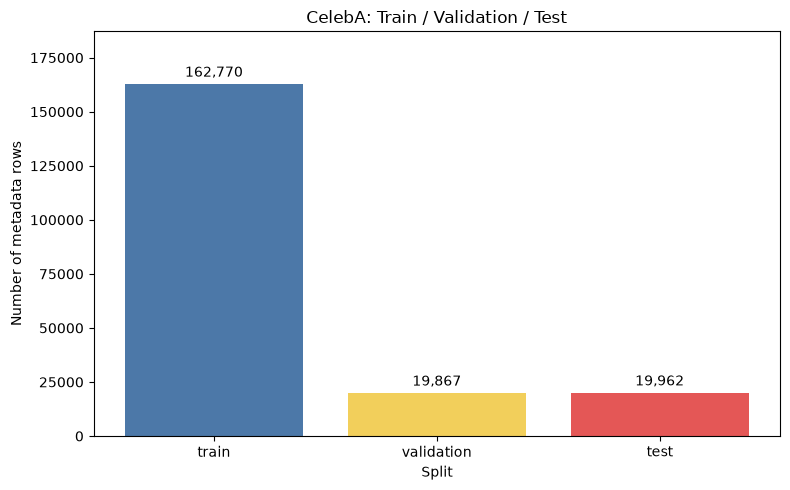
\includegraphics[width=\textwidth]{figures/eda_partitions.png}
    \caption{Official partition counts ($N = 202{,}599$).}
  \end{subfigure}
  \hfill
  \begin{subfigure}[b]{0.55\textwidth}
    \centering
    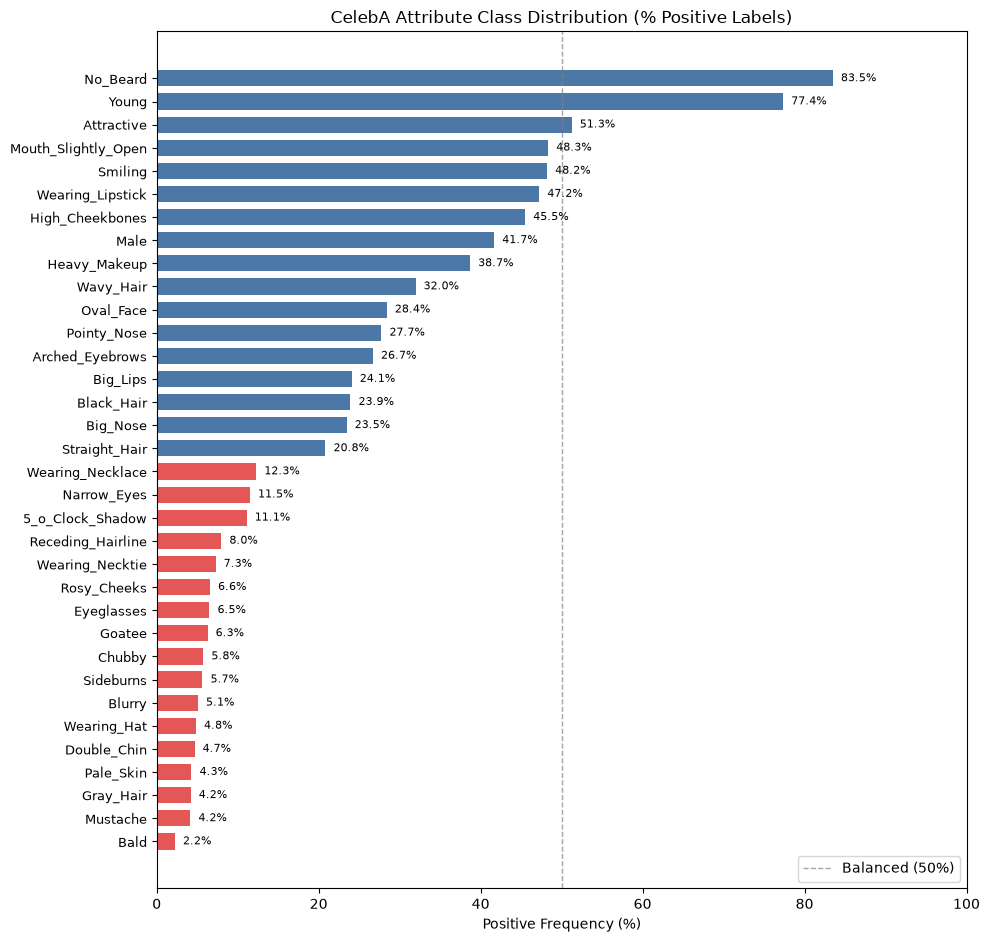
\includegraphics[width=\textwidth]{figures/eda_attribute_imbalance.png}
    \caption{Prevalence of 34 extreme attributes (17 highest, 17 lowest).}
  \end{subfigure}
  \caption[Official partition counts and 34-attribute class imbalance]{Full-dataset CelebA EDA from \code{notebooks/\allowbreak{}run\_\allowbreak{}vision.ipynb}: (a) official train/validation/test split sizes and (b) positive-label prevalence for 34 of the 40 attributes (the 17 most frequent and 17 rarest; red bars indicate rare attributes with $<20\%$ positive labels).}
  \label{fig:eda_partitions_imbalance}
\end{figure}

\begin{figure}[htbp]
  \centering
  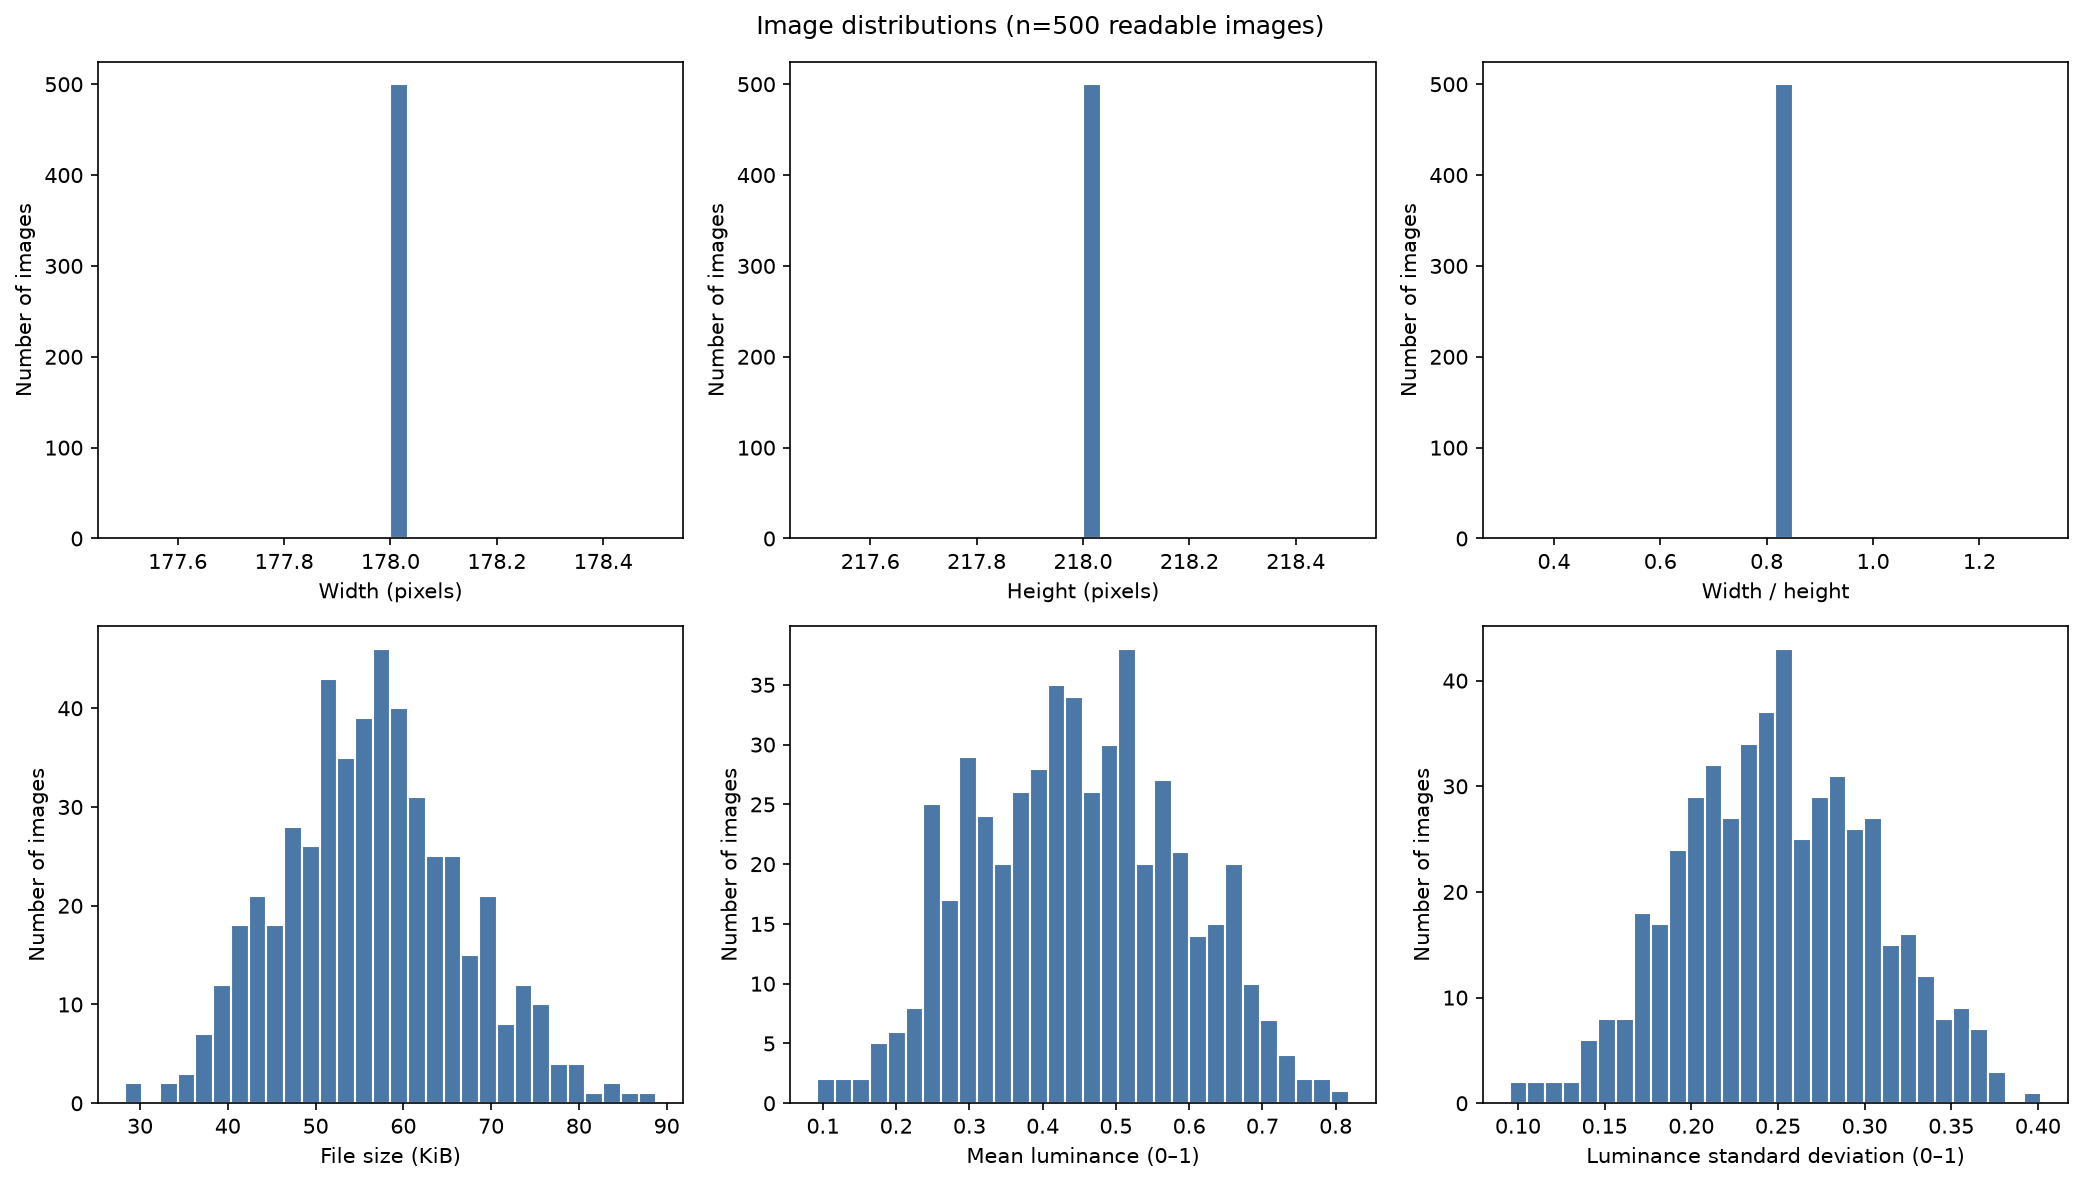
\includegraphics[width=0.84\textwidth]{figures/eda_image_distributions.png}
  \caption[Image dimension, file-size, and luminance distributions]{Distribution of image dimensions, aspect ratio, PNG file size, and luminance statistics over 500 deterministically sampled training images (\code{results/\allowbreak{}eda/\allowbreak{}image\_\allowbreak{}distributions.png}).}
  \label{fig:eda_image_dist}
\end{figure}

\begin{figure}[htbp]
  \centering
  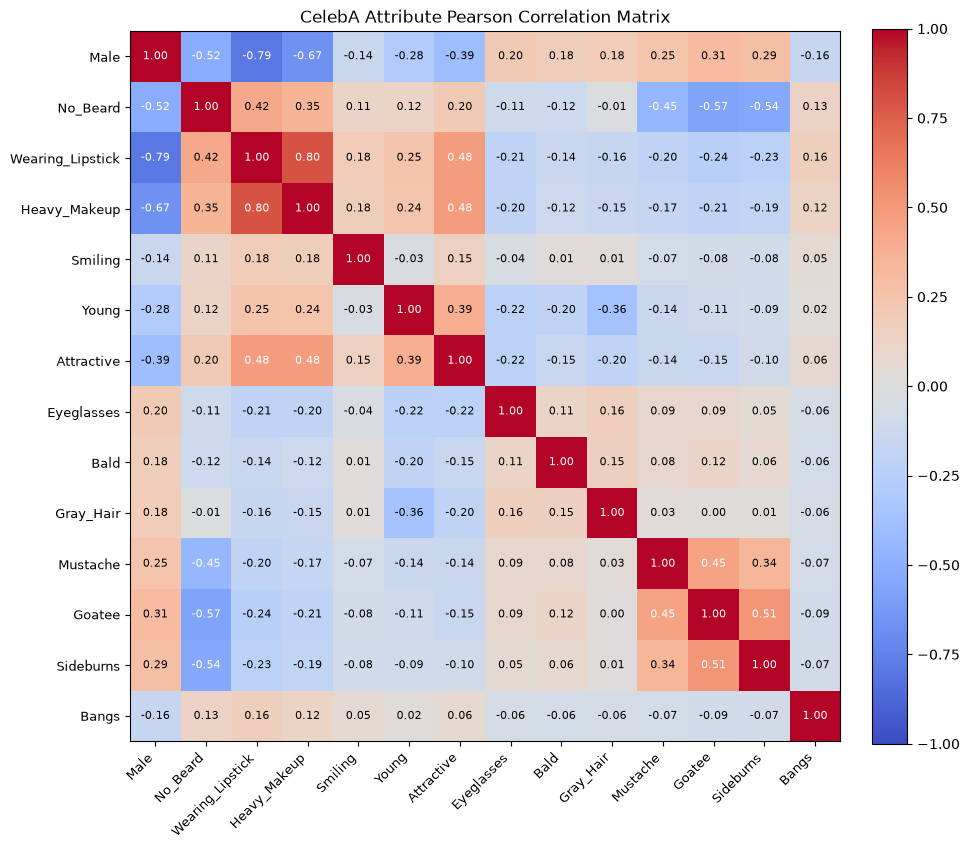
\includegraphics[width=0.72\textwidth]{figures/eda_attribute_correlations.png}
  \caption[Pairwise $\phi$-correlation heatmap across 14 key CelebA attributes]{Pairwise $\phi$-correlation heatmap across 14 key CelebA attributes (\code{notebooks/\allowbreak{}run\_\allowbreak{}vision.ipynb}, cell~32), highlighting strong co-occurrence among gender-associated facial cues.}
  \label{fig:eda_corr}
\end{figure}

\begin{figure}[htbp]
  \centering
  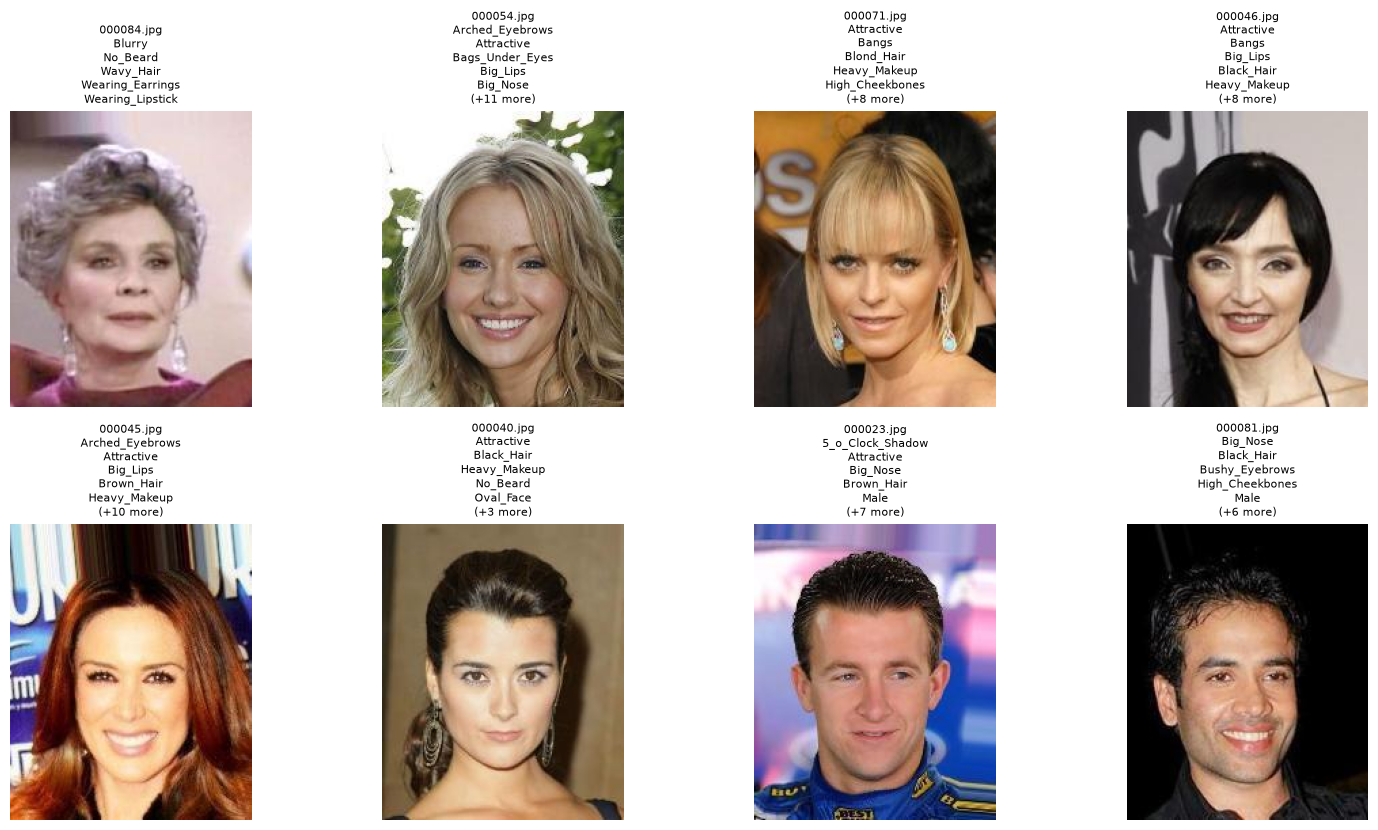
\includegraphics[width=0.92\textwidth]{figures/eda_sample_attributes.png}
  \caption[Random aligned CelebA face crops with active binary attributes]{Eight randomly sampled aligned face crops ($178 \times 218$\,px) annotated with up to five active positive binary attributes (\code{notebooks/\allowbreak{}run\_\allowbreak{}vision.ipynb}, cell~33).}
  \label{fig:eda_samples}
\end{figure}

\clearpage
\subsection{Target Attribute Selection and 28,000-Image Sampling Design}
\label{subsec:sampling}

Guided by our EDA findings, we selected three target attributes that test complementary visual scales and class-balance regimes:
\begin{enumerate}[leftmargin=20pt, itemsep=2pt]
  \item \textbf{\code{Smiling}} (near-balanced, $\approx 48\%$ positive): localized, fine-grained facial expression around the mouth and cheeks with known annotation subjectivity.
  \item \textbf{\code{Male}} (mildly imbalanced, $\approx 42\%$ train / $38\%$ test positive): holistic facial structure supported by strong global cues (hairline, facial hair, cosmetics).
  \item \textbf{\code{Eyeglasses}} (strongly imbalanced, $\approx 6.5\%$ positive, $\approx 15{:}1$ negative-to-positive ratio): localized object attribute around the eyes that rigorously exposes the failure of raw accuracy on rare classes.
\end{enumerate}

To balance statistical power with rapid, reproducible multi-backbone experimentation, \code{modules/\allowbreak{}vision/\allowbreak{}data/\allowbreak{}celeba.py} samples each official split independently using \code{seed = 42} to construct a 28,000-image manifest (\code{results/\allowbreak{}manifest.csv}): \textbf{20,000 train}, \textbf{4,000 validation}, and \textbf{4,000 test} images, deterministically sorted by \code{(partition, image\_\allowbreak{}id)} with labels mapped from $\{-1, 1\}$ to $\{0, 1\}$. As verified in Table~\ref{tab:subset_counts}, the sampled positive rates closely mirror the full-dataset prevalences, including the natural 4.40-percentage-point train-to-test drop in \code{Male} positive prevalence within the 28,000-image subset (42.55\% on train vs.\ 38.15\% on test, consistent with the 3.92-percentage-point validation-to-test shift on the full dataset).

\begin{table}[H]
  \centering
  \caption[Target class distribution in the 28,000-image subset]{Class distribution of the three target attributes in the 28,000-image experimental subset (\code{results/\allowbreak{}eda/\allowbreak{}class\_\allowbreak{}counts.csv}, \code{seed = 42}).}
  \label{tab:subset_counts}
  \small
  \begin{tabular}{@{}l r r r r r r r r r@{}}
    \toprule
    & \multicolumn{3}{c}{\textbf{Train ($n = 20{,}000$)}} & \multicolumn{3}{c}{\textbf{Validation ($n = 4{,}000$)}} & \multicolumn{3}{c}{\textbf{Test ($n = 4{,}000$)}} \\
    \cmidrule(lr){2-4} \cmidrule(lr){5-7} \cmidrule(lr){8-10}
    \textbf{Target} & \textbf{Neg} & \textbf{Pos} & \textbf{Pos \%} & \textbf{Neg} & \textbf{Pos} & \textbf{Pos \%} & \textbf{Neg} & \textbf{Pos} & \textbf{Pos \%} \\
    \midrule
    \code{Eyeglasses} & 18,701 & 1,299 & 6.50\%  & 3,730 & 270   & 6.75\%  & 3,751 & 249   & 6.23\% \\
    \code{Male}       & 11,491 & 8,509 & 42.55\% & 2,311 & 1,689 & 42.23\% & 2,474 & 1,526 & 38.15\% \\
    \code{Smiling}    & 10,466 & 9,534 & 47.67\% & 2,087 & 1,913 & 47.83\% & 2,023 & 1,977 & 49.43\% \\
    \bottomrule
  \end{tabular}
\end{table}

% --------------------------------------------------
\section{Methodology and Machine Learning Pipeline}
\label{sec:methodology}

\subsection{End-to-End Pipeline Architecture}
\label{subsec:pipeline_arch}

The system is implemented as a modular, configuration-driven Python package under \code{modules/\allowbreak{}vision/\allowbreak{}} orchestrated by \code{modules/\allowbreak{}vision/\allowbreak{}run.py} and parameterized via JSON (\code{configs/\allowbreak{}vision/\allowbreak{}celeba.json}). Figure~\ref{fig:pipeline_diagram} depicts the eight-stage workflow from raw CelebA files to final multi-model evaluation and prediction galleries. Every stage enforces strict row-order alignment against \code{manifest.csv} so that extracted feature matrices can be cached once per backbone and reused cleanly across all targets and classifiers.

\begin{figure}[H]
  \centering
  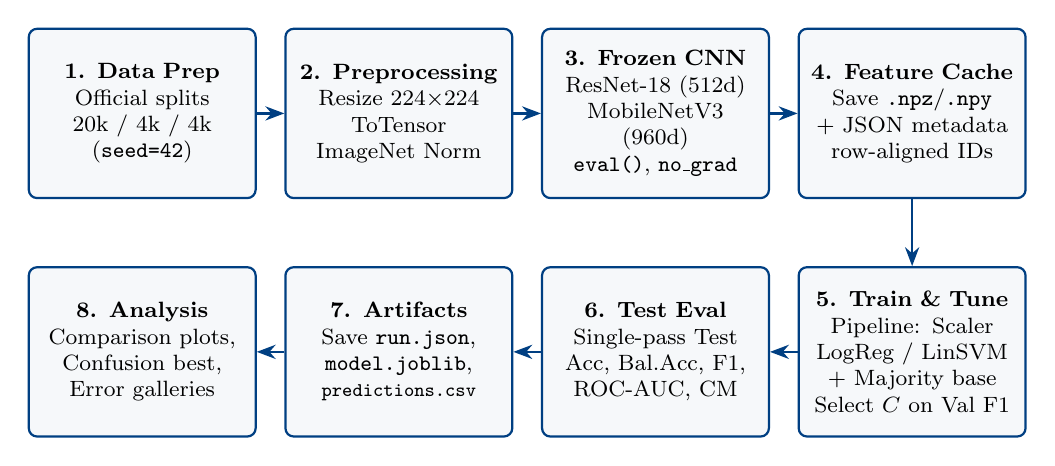
\begin{tikzpicture}[
    node distance=0.50cm and 0.35cm,
    box/.style={
      rectangle, rounded corners=3pt, draw=hcmutblue!85!black, thick,
      fill=lightgraybg, align=center, font=\footnotesize,
      minimum height=2.15cm, text width=2.60cm, inner sep=4pt
    },
    arrow/.style={-{Stealth[length=2.4mm]}, thick, color=hcmutblue!85!black}
  ]
    % Row 1
    \node[box] (data) {\textbf{1. Data Prep}\\Official splits\\20k / 4k / 4k\\(\code{seed=42})};
    \node[box, right=of data] (prep) {\textbf{2. Preprocessing}\\Resize $224{\times}224$\\ToTensor\\ImageNet Norm};
    \node[box, right=of prep] (feat) {\textbf{3. Frozen CNN}\\ResNet-18 (512d)\\MobileNetV3 (960d)\\\code{eval()}, \code{no\_\allowbreak{}grad}};
    \node[box, right=of feat] (store) {\textbf{4. Feature Cache}\\Save \code{.npz}/\code{.npy}\\+ JSON metadata\\row-aligned IDs};

    % Row 2
    \node[box, below=0.85cm of store] (train) {\textbf{5. Train \& Tune}\\Pipeline: Scaler\\LogReg / LinSVM\\+ Majority base\\Select $C$ on Val F1};
    \node[box, left=of train] (eval) {\textbf{6. Test Eval}\\Single-pass Test\\Acc, Bal.Acc, F1,\\ROC-AUC, CM};
    \node[box, left=of eval] (art) {\textbf{7. Artifacts}\\Save \code{run.json},\\\code{model.joblib},\\{\scriptsize\code{predictions.csv}}};
    \node[box, left=of art] (comp) {\textbf{8. Analysis}\\Comparison plots,\\Confusion best,\\Error galleries};

    \draw[arrow] (data) -- (prep);
    \draw[arrow] (prep) -- (feat);
    \draw[arrow] (feat) -- (store);
    \draw[arrow] (store) -- (train);
    \draw[arrow] (train) -- (eval);
    \draw[arrow] (eval) -- (art);
    \draw[arrow] (art) -- (comp);
  \end{tikzpicture}
  \caption[End-to-end modular vision classification pipeline]{End-to-end modular vision classification pipeline implemented in \code{modules/\allowbreak{}vision/\allowbreak{}run.py}. Features are extracted once per backbone and cached, while standardization and hyperparameter selection remain strictly isolated from the test split.}
  \label{fig:pipeline_diagram}
\end{figure}

\subsection{Image Preprocessing}
\label{subsec:preprocessing}

Implemented in \code{modules/\allowbreak{}vision/\allowbreak{}data/\allowbreak{}preprocessing.py}, each RGB image passes through three deterministic torchvision transforms:
\begin{enumerate}[leftmargin=20pt, itemsep=2pt]
  \item \textbf{Spatial resizing}: \code{Resize((224, 224))} maps the $218 \times 178$ aligned face crop directly to the canonical $224 \times 224$ input resolution of ImageNet-pretrained backbones. Although direct square resizing applies a modest horizontal stretch (aspect ratio $0.8165 \to 1.0$), it preserves the entire face frame rather than center-cropping away peripheral cues such as eyeglass temples, chin contours, or hairlines.
  \item \textbf{Tensor scaling}: \code{ToTensor()} rescales 8-bit pixel values from $[0, 255]$ to $[0.0, 1.0]$ in $(C, H, W)$ layout.
  \item \textbf{ImageNet normalization}: Channel-wise standardization using ImageNet statistics $\boldsymbol{\mu} = (0.485, 0.456, 0.406)$ and $\boldsymbol{\sigma} = (0.229, 0.224, 0.225)$ ensures input feature distributions match the pretrained convolutional filters.
\end{enumerate}

\subsection{Pretrained CNN Feature Extraction and Storage}
\label{subsec:feature_extraction}

Within \code{modules/\allowbreak{}vision/\allowbreak{}features/\allowbreak{}extraction.py}, pretrained backbones from \code{torchvision.models}~\cite{paszke2019pytorch} are loaded with their default ImageNet-1K weights, placed in inference mode (\code{model.eval()}), and executed under \code{torch.no\_\allowbreak{}grad()} with \code{shuffle=False} to preserve exact manifest ordering. The final classification layer is replaced by \code{nn.Identity()} so that global pooled penultimate representations are emitted directly:
\begin{itemize}[leftmargin=18pt, itemsep=2pt]
  \item \textbf{ResNet-18}~\cite{he2016resnet} (\code{ResNet18\_\allowbreak{}Weights.DEFAULT}, \code{model.fc = nn.Identity()}): A classic 18-layer residual network using skip connections across $3 \times 3$ convolutional blocks, producing a \textbf{512-dimensional} global average-pooled feature vector per image.
  \item \textbf{MobileNetV3-Large}~\cite{howard2019mobilenetv3} (\code{MobileNet\_\allowbreak{}V3\_\allowbreak{}Large\_\allowbreak{}Weights.DEFAULT}, \code{model.classifier = nn.Identity()}): A hardware-aware architecture discovered via neural architecture search combining inverted residual bottlenecks, depthwise separable convolutions, Squeeze-and-Excitation (SE) channel attention, and hard-swish activations, producing a \textbf{960-dimensional} pooled feature vector per image.
\end{itemize}

This backbone pair provides a meaningful architectural contrast---standard residual convolutions (512-d) versus attention-augmented inverted residuals (960-d)---while keeping feature extraction under 15 seconds per backbone on a single GPU. Extracted \code{float32} matrices are cached via \code{modules/\allowbreak{}vision/\allowbreak{}features/\allowbreak{}storage.py} as compressed \code{.npz} archives bundling \code{features}, \code{image\_\allowbreak{}ids}, \code{splits}, \code{labels}, and JSON metadata, and exported in the experiment bundle (\code{evaluation/\allowbreak{}bundle.py}) as standard \code{.npy} files (reopened with memory mapping, \code{mmap\_\allowbreak{}mode="r"}, during training) alongside JSON descriptors (\code{results/\allowbreak{}features/\allowbreak{}*.json}). Table~\ref{tab:extractors} summarizes both feature sets.

\begin{table}[H]
  \centering
  \caption[Comparison of pretrained CNN feature extractors]{Comparison of the two frozen pretrained CNN feature extractors on the 28,000-image subset (\code{results/\allowbreak{}features/\allowbreak{}*.json}, NVIDIA RTX~A4000, \code{batch\_\allowbreak{}size = 64}).}
  \label{tab:extractors}
  \footnotesize
  \setlength{\tabcolsep}{4.5pt}
  \begin{tabularx}{\textwidth}{@{}l Y r l r r@{}}
    \toprule
    \textbf{Backbone} & \textbf{Pretrained Weights} & \textbf{Dim ($d$)} & \textbf{Dtype} & \textbf{Size (MiB)} & \textbf{Time (s)} \\
    \midrule
    \code{resnet18} & \code{ResNet18\_\allowbreak{}Weights.DEFAULT} & 512 & \code{float32} & 54.69 & 14.06 \\
    \code{mobilenet\_\allowbreak{}v3\_\allowbreak{}large} & \code{MobileNet\_\allowbreak{}V3\_\allowbreak{}Large\_\allowbreak{}Weights.DEFAULT} & 960 & \code{float32} & 102.54 & 13.11 \\
    \bottomrule
  \end{tabularx}
\end{table}

\subsection{Classical Classifiers and Baseline Formulation}
\label{subsec:classifiers}

Penultimate representations from ImageNet-pretrained CNNs are typically well suited to linear separation, making regularized linear models strong, fast, and interpretable downstream classifiers~\cite{pedregosa2011scikit}. In \code{modules/\allowbreak{}vision/\allowbreak{}models/\allowbreak{}classification.py}, each backbone's feature matrix is evaluated with three models:

\begin{enumerate}[leftmargin=20pt, itemsep=3pt]
  \item \textbf{Majority Baseline (\code{DummyClassifier(strategy="most\_\allowbreak{}frequent")})}: Always predicts the most prevalent class in $\mathcal{D}_{\text{train}}$ (class \code{0} for all three attributes). It establishes a non-learning floor that exposes accuracy inflation on imbalanced targets.
  \item \textbf{L2-Regularized Logistic Regression (\code{LogisticRegression})}: Preceded by \code{StandardScaler}, fits weights $\mathbf{w} \in \mathbb{R}^{d}$ and intercept $b \in \mathbb{R}$ by minimizing the L2-regularized binary cross-entropy objective (Equation~\eqref{eq:logreg}):
  \begin{equation}
    \min_{\mathbf{w}, b} \; \frac{1}{2}\|\mathbf{w}\|_2^2 + C \sum_{i=1}^{n_{\text{train}}} \log\!\left(1 + \exp\!\left(-y'_i (\mathbf{w}^\top \tilde{\mathbf{x}}_i + b)\right)\right),
    \label{eq:logreg}
  \end{equation}
  where $y'_i \in \{-1, +1\}$ denotes the signed binary label, $\tilde{\mathbf{x}}_i$ is the standardized feature vector, and $C > 0$ is the inverse regularization strength (smaller $C$ imposes stronger shrinkage). Predicted probabilities $\hat{p}_i = \sigma(\mathbf{w}^\top \tilde{\mathbf{x}}_i + b)$ serve as continuous ranking scores for ROC-AUC.
  \item \textbf{Linear Support Vector Machine (\code{LinearSVC})}~\cite{fan2008liblinear}: Preceded by \code{StandardScaler}, minimizes the L2-regularized squared-hinge loss with \code{max\_\allowbreak{}iter = 10000} (Equation~\eqref{eq:linsvc}):
  \begin{equation}
    \min_{\mathbf{w}, b} \; \frac{1}{2}\|\mathbf{w}\|_2^2 + C \sum_{i=1}^{n_{\text{train}}} \max\!\left(0,\, 1 - y'_i (\mathbf{w}^\top \tilde{\mathbf{x}}_i + b)\right)^2.
    \label{eq:linsvc}
  \end{equation}
  Signed margin scores $s_i = \mathbf{w}^\top \tilde{\mathbf{x}}_i + b$ from \code{decision\_\allowbreak{}function} are used to compute ROC-AUC. Note that in \code{scikit-learn}'s LIBLINEAR backend with default \code{intercept\_\allowbreak{}scaling = 1.0}, the intercept $b$ is also regularized via $\frac{1}{2}(\|\mathbf{w}\|_2^2 + b^2)$.
\end{enumerate}

Feature standardization via \code{StandardScaler} ($\tilde{x}_{ij} = (x_{ij} - \mu_j)/\sigma_j$) ensures that the isotropic L2 penalty $\frac{1}{2}\|\mathbf{w}\|_2^2$ acts uniformly across all 512 or 960 embedding dimensions and accelerates solver convergence.

\subsection{Validation Protocol, Hyperparameter Tuning, and Leakage Prevention}
\label{subsec:leakage}

Model selection is governed by \code{modules/\allowbreak{}vision/\allowbreak{}training/\allowbreak{}classification.py} using three explicit safeguards against data leakage:
\begin{enumerate}[leftmargin=20pt, itemsep=2pt]
  \item \textbf{Split preservation}: Official CelebA partition codes are preserved verbatim during sampling; training, validation, and test indices never overlap.
  \item \textbf{In-pipeline standardization}: \code{StandardScaler} is encapsulated inside \code{sklearn.\allowbreak{}pipeline.\allowbreak{}Pipeline} alongside the classifier, guaranteeing that per-dimension means and standard deviations are estimated exclusively from $\mathcal{D}_{\text{train}}$ and only applied via \code{transform()} to $\mathcal{D}_{\text{val}}$ and $\mathcal{D}_{\text{test}}$.
  \item \textbf{Strict test-split isolation}: For both \code{LogisticRegression} and \code{LinearSVC}, the regularization strength is tuned over the six-point logarithmic grid
  \begin{equation*}
    C \in \{10^{-4},\; 10^{-3},\; 10^{-2},\; 10^{-1},\; 1.0,\; 10.0\}
  \end{equation*}
  by fitting on the 20,000 training embeddings and selecting the value maximizing \textbf{validation F1-score} on the 4,000 validation embeddings. The function \code{train\_\allowbreak{}classifier()} never reads test features or test labels---a guarantee verified automatically by the unit test \code{test\_\allowbreak{}train\_\allowbreak{}classifier\_\allowbreak{}does\_\allowbreak{}not\_\allowbreak{}leak\_\allowbreak{}test\_\allowbreak{}split}, which corrupts all test labels to \code{999} and asserts identical selected hyperparameters, validation metrics, and predictions on held-out feature rows. Similarly, \code{best\_\allowbreak{}runs()} in \code{evaluation/\allowbreak{}comparison.py} selects the winning configuration per target strictly by \code{val\_\allowbreak{}f1}.
\end{enumerate}

% --------------------------------------------------
\section{Experimental Setup and Evaluation Metrics}
\label{sec:setup}

\subsection{Experiment Matrix and Configuration Summary}
\label{subsec:exp_matrix}

The full experiment grid crosses 3 target attributes (\code{Eyeglasses}, \code{Male}, \code{Smiling}), 2 frozen feature extractors (\code{resnet18}, \code{mobilenet\_\allowbreak{}v3\_\allowbreak{}large}), and 3 classifiers (\code{majority}, \code{logistic\_\allowbreak{}regression}, \code{linear\_\allowbreak{}svc}), yielding \textbf{18 evaluated configurations}. Because each of the 12 learned configurations searches 6 values of $C$ on the validation split, the complete study executes 72 parameterized training trials plus 6 baseline fits. Table~\ref{tab:exp_setup} consolidates all fixed settings recorded in \code{results/\allowbreak{}config.json}.

\begin{table}[H]
  \centering
  \caption[Experimental configuration and execution environment]{Experimental configuration and execution environment verified from \code{results/\allowbreak{}config.json}, \code{results/\allowbreak{}gpu.csv}, \code{pyproject.toml}, and classifier/training defaults in \code{modules/\allowbreak{}vision/\allowbreak{}\{models,training\}/\allowbreak{}classification.py}.}
  \label{tab:exp_setup}
  \small
  \begin{tabularx}{\textwidth}{@{}l Y@{}}
    \toprule
    \textbf{Setting Category} & \textbf{Verified Value / Specification} \\
    \midrule
    Target Attributes & \code{Smiling}, \code{Male}, \code{Eyeglasses} (3 independent binary tasks) \\
    Dataset Split Sizes & Train: 20,000 \,/\, Validation: 4,000 \,/\, Test: 4,000 (total 28,000; official partitions) \\
    Random Seed & \code{seed = 42} (sampling and classifier initialization) \\
    Image Transform & \code{Resize(224, 224)} + \code{ToTensor()} + ImageNet mean/std normalization \\
    Feature Extractors & \code{resnet18} (512-d), \code{mobilenet\_\allowbreak{}v3\_\allowbreak{}large} (960-d); \code{batch\_\allowbreak{}size = 64}, \code{num\_\allowbreak{}workers = 8} \\
    Classifiers & \code{majority} (\code{DummyClassifier}), \code{logistic\_\allowbreak{}regression} (\code{max\_\allowbreak{}iter=1000}), \code{linear\_\allowbreak{}svc} (\code{max\_\allowbreak{}iter=10000}) \\
    Hyperparameter Grid & $C \in \{10^{-4}, 10^{-3}, 10^{-2}, 10^{-1}, 1.0, 10.0\}$; selection metric: \code{val\_\allowbreak{}f1} \\
    Hardware (GPU Run) & NVIDIA RTX A4000 (16,376 MiB VRAM), Driver \code{580.178.04} (via Vast.ai, \code{scripts/\allowbreak{}vast\_\allowbreak{}run.sh}) \\
    Software Stack & Python $\ge 3.11$, PyTorch $\ge 2.3$, Torchvision $\ge 0.18$, scikit-learn $\ge 1.5$, NumPy $\ge 2.0$, pandas $\ge 2.2$ \\
    Tracked Git Commit & \code{0bb3bc0534da8323c9d9af71b3bdde43fd7320d8} (merged to \code{origin/\allowbreak{}main} at \code{6ddb47e}) \\
    \bottomrule
  \end{tabularx}
\end{table}

\subsection{Reproducibility and Automated Testing}
\label{subsec:reproducibility}

Reproducibility is enforced at three levels: (i)~every standard run of \code{modules/\allowbreak{}vision/\allowbreak{}run.py} writes \code{manifest.csv}, a per-configuration \code{run.json} (recording all validation \code{trials}), \code{metrics.json}, fitted \code{model.joblib}, \code{predictions.csv}, summary comparison tables, and figures/galleries to \code{results/\allowbreak{}}; enabling \code{--export-bundle} additionally writes \code{config.json}, \code{validation\_\allowbreak{}predictions.csv}, \code{eda/}, \code{features/\allowbreak{}*.npy}, and \code{comparison\_\allowbreak{}crops/}, while the remote GPU runner (\code{scripts/\allowbreak{}vast\_\allowbreak{}run.sh}) captures \code{git\_\allowbreak{}commit.txt} and \code{gpu.csv}; (ii)~\code{run.py} supports \code{--reference-manifest} to assert exact sample-ID, split, and label equality across re-runs; and (iii)~two automated \code{pytest} suites (\code{tests/\allowbreak{}test\_\allowbreak{}vision\_\allowbreak{}classification.py} and \code{tests/\allowbreak{}test\_\allowbreak{}vision\_\allowbreak{}pipeline.py}) validate data preparation, feature alignment, model building, end-to-end execution on a synthetic dataset, and test-label isolation.

\textbf{Notebook and Google Colab front-end.} In \code{notebooks/\allowbreak{}run\_\allowbreak{}vision.ipynb}, cells~1--33 preserve the executed full-dataset EDA outputs on Kaggle CelebA, whereas cells~35--41 provide interactive entry points calling \code{run\_\allowbreak{}eda()} and \code{run\_\allowbreak{}pipeline()}. The 18-configuration RTX~A4000 benchmark reported in this paper was executed non-interactively via \code{scripts/\allowbreak{}vast\_\allowbreak{}run.sh} by downloading the public mirror \code{flwrlabs/\allowbreak{}celeba} without mounting personal cloud drives; for standalone Google Colab \code{Runtime -> Run all} execution, cells~35--41 only require installing dependencies (\code{requirements.txt}) and invoking \code{scripts/\allowbreak{}download\_\allowbreak{}celeba.py --data-dir data} beforehand.

\subsection{Evaluation Metrics}
\label{subsec:metrics}

Let $\text{TP}$, $\text{FP}$, $\text{FN}$, and $\text{TN}$ denote true positives, false positives, false negatives, and true negatives on $\mathcal{D}_{\text{test}}$. We report six complementary binary classification metrics implemented in \code{modules/\allowbreak{}vision/\allowbreak{}evaluation/\allowbreak{}classification.py} (Equations~\eqref{eq:acc_balacc}--\eqref{eq:f1}):
\begin{align}
  \text{Accuracy} &= \frac{\text{TP} + \text{TN}}{\text{TP} + \text{TN} + \text{FP} + \text{FN}}, &
  \text{Balanced Accuracy} &= \frac{1}{2}\!\left(\frac{\text{TP}}{\text{TP} + \text{FN}} + \frac{\text{TN}}{\text{TN} + \text{FP}}\right), \label{eq:acc_balacc} \\
  \text{Precision} &= \frac{\text{TP}}{\text{TP} + \text{FP}}, &
  \text{Recall} &= \frac{\text{TP}}{\text{TP} + \text{FN}}, \label{eq:pr} \\
  \text{F1} &= \frac{2 \cdot \text{Precision} \cdot \text{Recall}}{\text{Precision} + \text{Recall}}. \label{eq:f1}
\end{align}
In addition, \textbf{ROC-AUC} measures the area under the Receiver Operating Characteristic curve across all classification thresholds using continuous model scores (\code{predict\_\allowbreak{}proba[:, 1]} for Logistic Regression, \code{decision\_\allowbreak{}function} for LinearSVC).

\textbf{Metric rationale.} On \code{Eyeglasses} (only 6.23\% positive samples in the test split), a trivial majority classifier achieves 93.78\% raw accuracy while detecting zero positive cases ($\text{Recall} = 0$, $\text{F1} = 0$, $\text{Balanced Accuracy} = 0.50$). Consequently, \textbf{F1-score} is adopted as the primary selection and comparison metric because it directly penalizes both missed detections and false alarms on the positive class, while \textbf{Balanced Accuracy} and \textbf{ROC-AUC} separate threshold-dependent behavior from underlying ranking separability.

% --------------------------------------------------
\section{Experimental Results and Analysis}
\label{sec:results}

\subsection{Overall Quantitative Comparison Across All 18 Configurations}
\label{subsec:overall_results}

Table~\ref{tab:main_results} compiles the validation F1-score, selected regularization constant $C$, and all six test-set metrics across all 18 configurations from \code{results/\allowbreak{}comparison.csv}. Figures~\ref{fig:comp_f1} and~\ref{fig:comp_auc} visualize the grouped test F1-score and ROC-AUC comparisons side by side. (In tables and figures below, \code{MobileNetV3}, \code{LogReg}, and \code{LinSVM} abbreviate \code{MobileNetV3-Large}, \code{LogisticRegression}, and \code{LinearSVC}, respectively.)

\begin{table}[H]
  \centering
  \caption[Quantitative results across all 18 configurations]{Complete quantitative results across all 18 configurations ($n_{\text{val}} = 4{,}000$, $n_{\text{test}} = 4{,}000$, \code{seed = 42}). \textbf{Bold} rows mark the winning configuration per target selected strictly by \code{Val F1}.}
  \label{tab:main_results}
  \scriptsize
  \setlength{\tabcolsep}{3.4pt}
  \begin{tabular}{@{}l l l r r r r r r r r@{}}
    \toprule
    \textbf{Target} & \textbf{Extractor} & \textbf{Classifier} & \textbf{Best $C$} & \textbf{Val F1 $\uparrow$} & \textbf{Acc $\uparrow$} & \textbf{Bal.Acc $\uparrow$} & \textbf{Prec $\uparrow$} & \textbf{Rec $\uparrow$} & \textbf{Test F1 $\uparrow$} & \textbf{AUC $\uparrow$} \\
    \midrule
    \multirow{6}{*}{\code{Eyeglasses}}
      & \textbf{MobileNetV3} & \textbf{LinearSVC} & \textbf{0.001} & \textbf{0.8285} & \textbf{0.9792} & \textbf{0.8465} & \textbf{0.9611} & \textbf{0.6948} & \textbf{0.8065} & \textbf{0.9774} \\
      & MobileNetV3 & LogReg    & 0.01  & 0.8167 & 0.9775 & 0.8455 & 0.9251 & 0.6948 & 0.7936 & 0.9778 \\
      & MobileNetV3 & Majority  & ---   & 0.0000 & 0.9378 & 0.5000 & 0.0000 & 0.0000 & 0.0000 & 0.5000 \\
      & ResNet-18   & LinearSVC & 0.01  & 0.7617 & 0.9728 & 0.8261 & 0.8723 & 0.6586 & 0.7506 & 0.9607 \\
      & ResNet-18   & LogReg    & 0.01  & 0.7692 & 0.9738 & 0.8173 & 0.9138 & 0.6386 & 0.7518 & 0.9639 \\
      & ResNet-18   & Majority  & ---   & 0.0000 & 0.9378 & 0.5000 & 0.0000 & 0.0000 & 0.0000 & 0.5000 \\
    \midrule
    \multirow{6}{*}{\code{Male}}
      & \textbf{MobileNetV3} & \textbf{LinearSVC} & \textbf{0.001} & \textbf{0.9329} & \textbf{0.9370} & \textbf{0.9361} & \textbf{0.9052} & \textbf{0.9325} & \textbf{0.9187} & \textbf{0.9844} \\
      & MobileNetV3 & LogReg    & 0.001 & 0.9318 & 0.9328 & 0.9318 & 0.8990 & 0.9279 & 0.9133 & 0.9835 \\
      & MobileNetV3 & Majority  & ---   & 0.0000 & 0.6185 & 0.5000 & 0.0000 & 0.0000 & 0.0000 & 0.5000 \\
      & ResNet-18   & LinearSVC & 0.01  & 0.9240 & 0.9238 & 0.9230 & 0.8847 & 0.9201 & 0.9020 & 0.9762 \\
      & ResNet-18   & LogReg    & 0.01  & 0.9218 & 0.9222 & 0.9212 & 0.8838 & 0.9168 & 0.9000 & 0.9763 \\
      & ResNet-18   & Majority  & ---   & 0.0000 & 0.6185 & 0.5000 & 0.0000 & 0.0000 & 0.0000 & 0.5000 \\
    \midrule
    \multirow{6}{*}{\code{Smiling}}
      & MobileNetV3 & LinearSVC & 0.001 & 0.7951 & 0.7980 & 0.7980 & 0.7965 & 0.7941 & 0.7953 & 0.8785 \\
      & \textbf{MobileNetV3} & \textbf{LogReg} & \textbf{0.01} & \textbf{0.7959} & \textbf{0.7985} & \textbf{0.7985} & \textbf{0.7962} & \textbf{0.7962} & \textbf{0.7962} & \textbf{0.8781} \\
      & MobileNetV3 & Majority  & ---   & 0.0000 & 0.5058 & 0.5000 & 0.0000 & 0.0000 & 0.0000 & 0.5000 \\
      & ResNet-18   & LinearSVC & 0.01  & 0.7798 & 0.7748 & 0.7746 & 0.7802 & 0.7577 & 0.7688 & 0.8573 \\
      & ResNet-18   & LogReg    & 0.1   & 0.7794 & 0.7752 & 0.7751 & 0.7799 & 0.7597 & 0.7697 & 0.8571 \\
      & ResNet-18   & Majority  & ---   & 0.0000 & 0.5058 & 0.5000 & 0.0000 & 0.0000 & 0.0000 & 0.5000 \\
    \bottomrule
  \end{tabular}
\end{table}

\textbf{Validation-to-test generalization.} Validation selection transfers reliably to the unseen test split across all three tasks. On \code{Smiling}, validation and test F1 are nearly identical (0.7959 vs.\ 0.7962 for MobileNetV3 + LogReg). On \code{Male}, test F1 (0.9187) trails validation F1 (0.9329) by 1.42 percentage points, which is consistent with the natural test-split drop in male prevalence observed during EDA (Section~\ref{subsec:eda_findings}: 42.23\% on validation vs.\ 38.15\% on test, causing a lower positive-class precision under a fixed decision boundary). On \code{Eyeglasses}, test F1 (0.8065) is 2.20 points below validation F1 (0.8285), reflecting higher sampling variance over the small positive cohort ($n_{\text{pos}} = 270$ on validation and $249$ on test), where recall shifts from 0.7333 to 0.6948.

\begin{figure}[htbp]
  \centering
  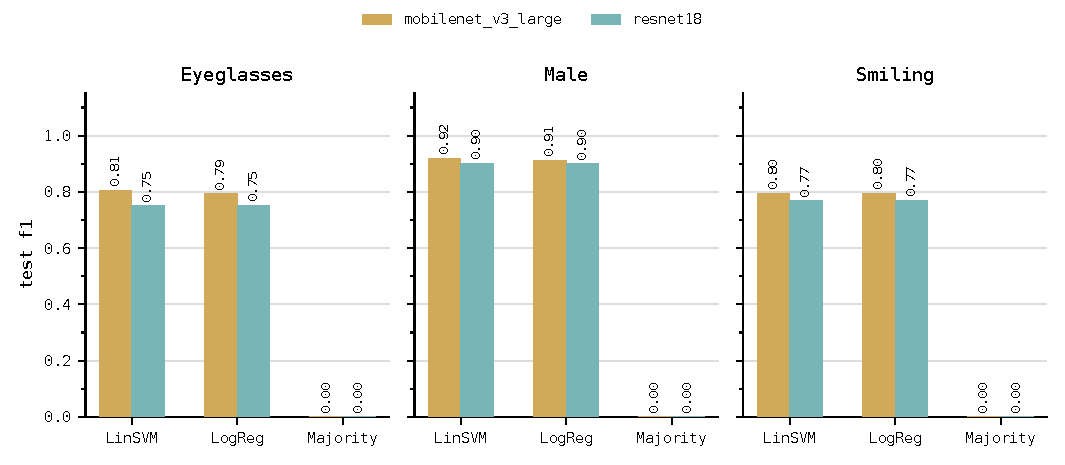
\includegraphics[width=0.92\textwidth]{figures/comparison_test_f1.pdf}
  \caption[Test-set F1-score comparison across all configurations]{Grouped bar chart of test-set F1-score across targets, feature extractors, and classifiers ($n_{\text{test}} = 4{,}000$; \code{results/\allowbreak{}figures/\allowbreak{}comparison\_\allowbreak{}test\_\allowbreak{}f1.pdf}).}
  \label{fig:comp_f1}
\end{figure}

\begin{figure}[htbp]
  \centering
  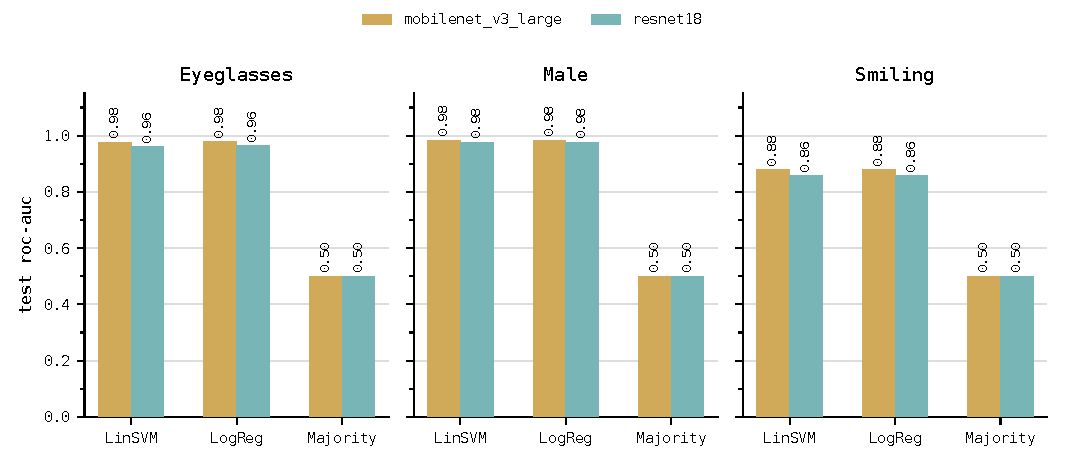
\includegraphics[width=0.92\textwidth]{figures/comparison_test_roc_auc.pdf}
  \caption[Test-set ROC-AUC comparison across all configurations]{Grouped bar chart of test-set ROC-AUC across targets, feature extractors, and classifiers ($n_{\text{test}} = 4{,}000$; \code{results/\allowbreak{}figures/\allowbreak{}comparison\_\allowbreak{}test\_\allowbreak{}roc\_\allowbreak{}auc.pdf}).}
  \label{fig:comp_auc}
\end{figure}

\subsection{Hyperparameter Sensitivity Analysis (Regularization Strength \texorpdfstring{$C$}{C})}
\label{subsec:c_sensitivity}

Figure~\ref{fig:c_sensitivity} plots validation F1 across all six tested values of $C \in \{10^{-4}, 10^{-3}, 10^{-2}, 10^{-1}, 1, 10\}$ for every parameterized configuration (full numerical tables are provided in Appendix~\ref{app:tuning}). Three consistent patterns emerge:
\begin{itemize}[leftmargin=18pt, itemsep=2pt]
  \item \textbf{Strong regularization is essential in 512--960 dimensions}: Eleven of the twelve learned configurations peak at $C = 0.001$ or $C = 0.01$; the sole exception (\code{ResNet-18 + LogReg} on \code{Smiling}) peaks marginally at $C = 0.1$ (0.7794 vs.\ 0.7783 at $C = 0.01$).
  \item \textbf{Underfitting at $C = 10^{-4}$}: Over-regularization severely depresses \code{LogisticRegression} on rare-class \code{Eyeglasses} (validation F1 collapses to 0.2848 on MobileNetV3 and 0.2965 on ResNet-18) because heavy L2 shrinkage pulls logits toward the negative prior, pushing most positive samples below the 0.5 probability threshold. \code{LinearSVC} degrades more gracefully at $C = 10^{-4}$ (0.7289 and 0.6015).
  \item \textbf{Overfitting at weak regularization ($C \ge 0.1$)}: On the higher-dimensional 960-d MobileNetV3 features, increasing $C$ from 0.001 to 10.0 causes \code{Eyeglasses} validation F1 to fall from 0.8285 to 0.7129 ($-11.56$ points) for \code{LinearSVC} and from 0.8167 ($C=0.01$) to 0.7270 ($-8.97$ points) for \code{LogisticRegression}. Expanding the tuning grid downward into $[10^{-4}, 10^{-2}]$ therefore yielded substantial generalization gains that a narrow default grid ($[0.1, 1, 10]$) would have missed.
\end{itemize}

\begin{figure}[H]
  \centering
  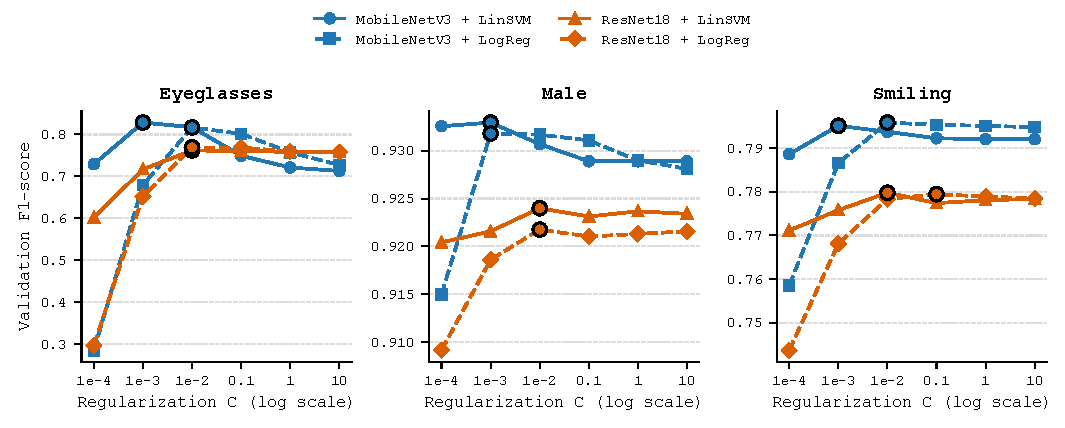
\includegraphics[width=0.96\textwidth]{figures/c_sensitivity.pdf}
  \caption[Validation F1-score sensitivity to regularization strength C]{Validation F1-score sensitivity to the inverse regularization strength $C$ (log scale) across all 12 parameterized configurations. Black-outlined markers denote the selected optimum per curve.}
  \label{fig:c_sensitivity}
\end{figure}

\subsection{Backbone Comparison: MobileNetV3-Large vs.\ ResNet-18}
\label{subsec:backbone_comp}

Holding the classifier and dataset split fixed, \textbf{MobileNetV3-Large dominates ResNet-18 in all six paired comparisons} (3 targets $\times$ 2 linear classifiers):
\begin{itemize}[leftmargin=18pt, itemsep=2pt]
  \item On \code{Eyeglasses}, MobileNetV3-Large improves test F1 by \textbf{+5.59 points} with LinearSVC (0.8065 vs.\ 0.7506) and \textbf{+4.18 points} with Logistic Regression (0.7936 vs.\ 0.7518), while lifting ROC-AUC by $+1.39$ to $+1.67$ points.
  \item On \code{Male}, MobileNetV3-Large improves test F1 by \textbf{+1.67 points} with LinearSVC (0.9187 vs.\ 0.9020) and \textbf{+1.33 points} with Logistic Regression (0.9133 vs.\ 0.9000).
  \item On \code{Smiling}, MobileNetV3-Large improves test F1 by \textbf{+2.65 points} on both LinearSVC (0.7953 vs.\ 0.7688) and Logistic Regression (0.7962 vs.\ 0.7697), with ROC-AUC gains exceeding $+2.1$ points.
\end{itemize}

\textbf{Interpretation and resource trade-off.} Two architectural factors plausibly explain MobileNetV3-Large's consistent edge: (i)~its penultimate representation provides nearly twice the feature capacity (960-d vs.\ 512-d), preserving finer localized visual descriptors (such as thin eyeglass frames and mouth-corner curvature), and (ii)~its Squeeze-and-Excitation channel-attention blocks and higher ImageNet-1K pretraining accuracy (\code{MobileNet\_\allowbreak{}V3\_\allowbreak{}Large\_\allowbreak{}Weights.IMAGENET1K\_\allowbreak{}V2} reaches 75.27\% top-1 vs.\ 69.76\% for \code{ResNet18\_\allowbreak{}Weights.IMAGENET1K\_\allowbreak{}V1} in \code{torchvision}~\cite{paszke2019pytorch}) produce more discriminative semantic channels. Practically, this accuracy gain comes with \emph{lower} extraction wall-clock time on the RTX~A4000 (13.11\,s vs.\ 14.06\,s for 28,000 images); the only trade-off is a $1.88\times$ larger feature footprint on disk (102.54\,MiB vs.\ 54.69\,MiB), which remains modest for modern workflows.

\subsection{Classifier Comparison: LinearSVC vs.\ Logistic Regression vs.\ Majority}
\label{subsec:classifier_comp}

Every learned linear model dramatically outperforms the \code{Majority} baseline on F1-score (from 0.0000 to 0.75--0.92) and Balanced Accuracy (from 0.5000 to 0.77--0.94). The \code{Eyeglasses} baseline sharply illustrates the \emph{accuracy paradox}: predicting ``no eyeglasses'' on all 4,000 test images yields 93.78\% accuracy yet detects 0 of 249 eyeglass wearers.

Comparing the two linear classifiers on the same backbone reveals far smaller gaps than switching backbones:
\begin{itemize}[leftmargin=18pt, itemsep=2pt]
  \item Using MobileNetV3-Large features, \code{LinearSVC} edges out \code{LogisticRegression} on \code{Eyeglasses} (0.8065 vs.\ 0.7936, $+1.29$ points, primarily via higher precision 0.9611 vs.\ 0.9251) and on \code{Male} (0.9187 vs.\ 0.9133, $+0.54$ points).
  \item On \code{Smiling}, \code{LogisticRegression} achieves a negligible lead (0.7962 vs.\ 0.7953, $+0.09$ points) while retaining the practical benefit of native probability estimates.
  \item Across all pairs, ROC-AUC differences between \code{LinearSVC} and \code{LogisticRegression} remain at most 0.0033, confirming that \textbf{representation quality (backbone choice) is the primary performance driver} in this frozen-feature regime.
\end{itemize}

\subsection{Confusion Matrices and Qualitative Error Analysis}
\label{subsec:error_analysis}

Table~\ref{tab:confusion_summary} and Figure~\ref{fig:confusion_best} detail the test-set confusion matrices of the three validation-selected best configurations, while Figures~\ref{fig:gallery_eyeglasses}--\ref{fig:gallery_Smiling} display representative true positives/negatives alongside the six most confident false positives and false negatives per attribute.

\begin{table}[H]
  \centering
  \caption[Test-set confusion counts for the best model per target]{Test-set confusion counts ($n_{\text{test}} = 4{,}000$) and per-class rates for the validation-selected best model per target.}
  \label{tab:confusion_summary}
  \footnotesize
  \setlength{\tabcolsep}{4.5pt}
  \begin{tabular}{@{}l l r r r r r r@{}}
    \toprule
    \textbf{Target} & \textbf{Best Model (Val-Selected)} & \textbf{TN} & \textbf{FP} & \textbf{FN} & \textbf{TP} & \textbf{TNR (Spec.)} & \textbf{TPR (Rec.)} \\
    \midrule
    \code{Eyeglasses} & MobileNetV3 + LinearSVC ($C{=}0.001$) & 3,744 & 7   & 76  & 173   & 99.81\% & 69.48\% \\
    \code{Male}       & MobileNetV3 + LinearSVC ($C{=}0.001$) & 2,325 & 149 & 103 & 1,423 & 93.98\% & 93.25\% \\
    \code{Smiling}    & MobileNetV3 + LogReg ($C{=}0.01$)     & 1,620 & 403 & 403 & 1,574 & 80.08\% & 79.62\% \\
    \bottomrule
  \end{tabular}
\end{table}

\begin{figure}[H]
  \centering
  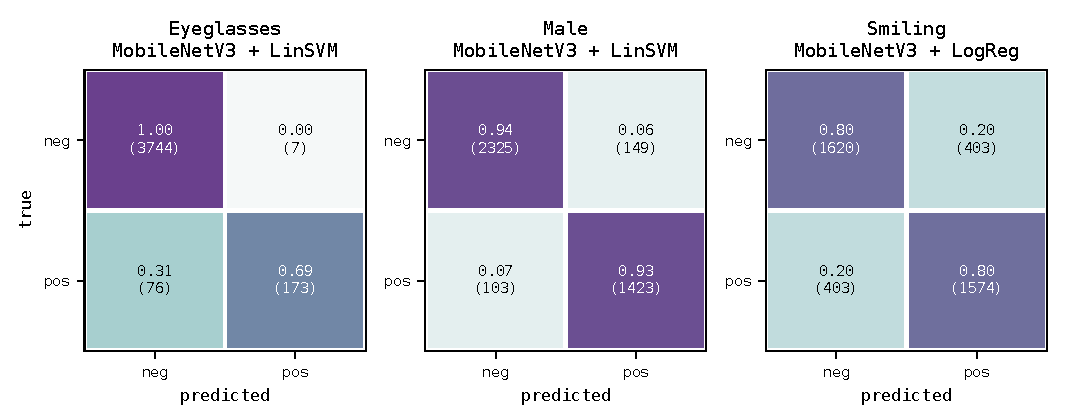
\includegraphics[width=0.92\textwidth]{figures/confusion_best.pdf}
  \caption[Row-normalized test-set confusion matrices of best models]{Row-normalized test-set confusion matrices ($n = 4{,}000$) for the best configuration per attribute selected by validation F1 (\code{results/\allowbreak{}figures/\allowbreak{}confusion\_\allowbreak{}best.pdf}).}
  \label{fig:confusion_best}
\end{figure}

\textbf{1. \code{Eyeglasses} --- strong precision--recall asymmetry and label noise (Figure~\ref{fig:gallery_eyeglasses}).}
Although the model achieves 0.9774 ROC-AUC and 99.81\% specificity (only 7 false positives out of 3,751 negative faces), it misses \textbf{76 of 249} eyeglass wearers (Recall = 69.48\%). Because ROC-AUC is near ceiling, the bottleneck is largely a conservative default decision threshold ($s = 0$) induced by the 15:1 class imbalance without class weighting or threshold tuning. Direct visual inspection of the gallery exposes four concrete failure mechanisms:
\begin{itemize}[leftmargin=18pt, itemsep=1.5pt]
  \item \emph{Rimless and thin wire-frame glasses} (FN samples \code{196691.png} at $-1.14$ and \code{201282.png} at $-1.05$): low-contrast metallic/transparent frames blend into skin texture after global pooling.
  \item \emph{Severe occlusion and dark shadows} (FN \code{187076.png} at $-2.63$ with a forearm covering the eye region; FN \code{197952.png} at $-1.21$ where dark sunglasses merge into dense hair and hat brim shadows).
  \item \emph{Visual distractors mimicking eyewear} (FP \code{190774.png} at $+0.55$ with heavy dark theatrical eye makeup; FP \code{191983.png} at $+0.48$ with sunglasses resting on a baseball cap brim; FP \code{193049.png} at $+0.07$ where a background person on the right edge wears sunglasses).
  \item \emph{CelebA ground-truth label noise}: Notably, two of the top six false positives (\code{199410.png} wearing white 3D glasses and \code{186787.png} wearing blue-tinted sunglasses) clearly depict eyewear despite negative ground-truth labels, while two top false negatives (\code{193705.png}, \code{201701.png}) show bare faces with no visible glasses.
\end{itemize}

\begin{figure}[H]
  \centering
  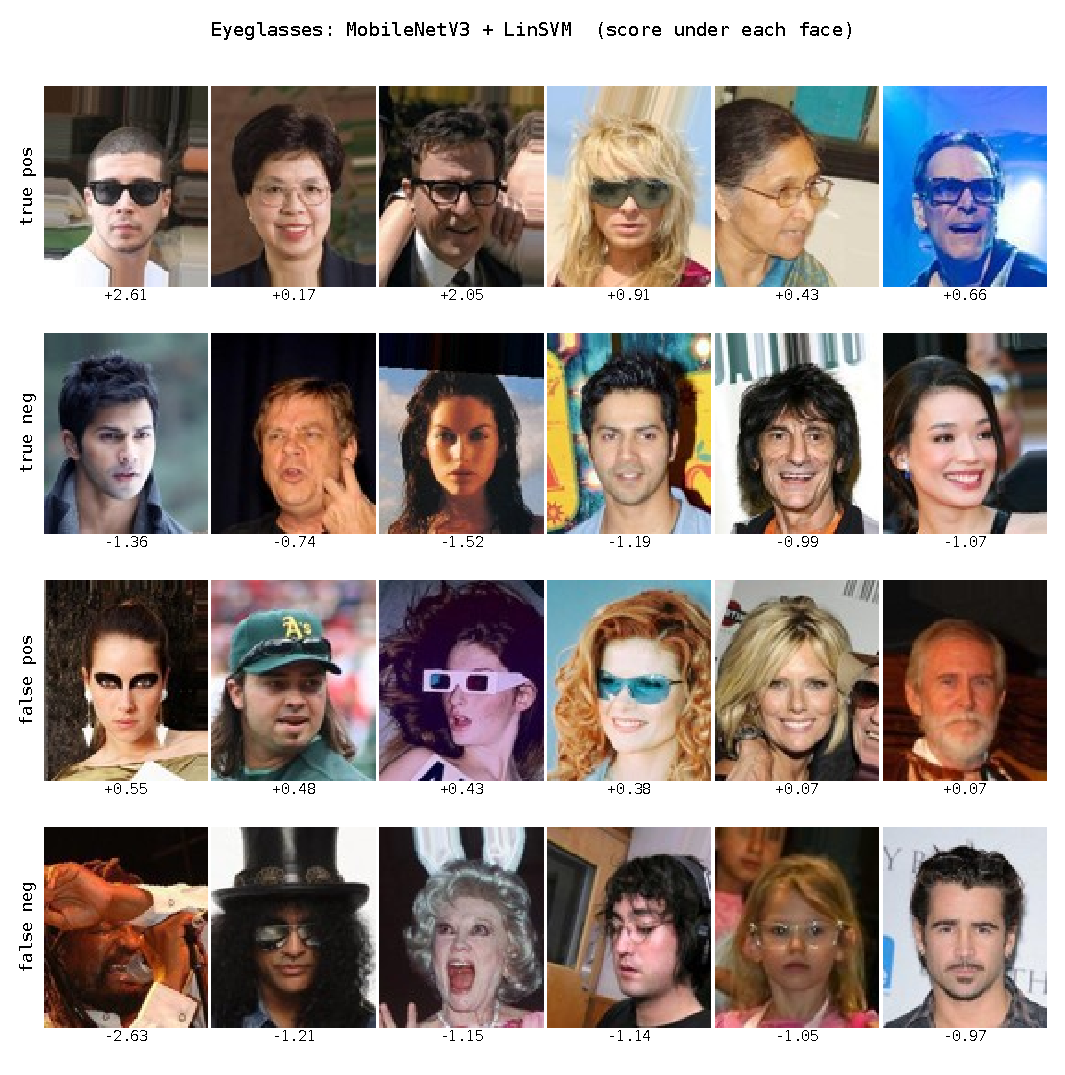
\includegraphics[width=0.84\textwidth]{figures/gallery_Eyeglasses.pdf}
  \caption[Qualitative prediction gallery for Eyeglasses]{Qualitative prediction gallery for \code{Eyeglasses} (\code{MobileNetV3 + LinearSVC}). Top two rows show random TP/TN test faces; bottom two rows show the six highest-confidence FP and FN errors with signed margin scores (\code{results/\allowbreak{}figures/\allowbreak{}gallery\_\allowbreak{}Eyeglasses.pdf}).}
  \label{fig:gallery_eyeglasses}
\end{figure}

\textbf{2. \code{Male} --- reliance on hairstyle and headwear shortcuts (Figure~\ref{fig:gallery_Male}).}
\code{Male} attains the strongest overall metrics (F1 = 0.9187, ROC-AUC = 0.9844) with balanced specificity (93.98\%) and sensitivity (93.25\%). Visual inspection shows that high-confidence errors follow clear gender-presentation heuristics---including cosmetic and facial-hair cues correlated with \code{Male} in EDA alongside visually prominent headwear and hairstyle cues:
\begin{itemize}[leftmargin=18pt, itemsep=1.5pt]
  \item \emph{False positives} (female faces predicted male, scores $+1.16$ to $+1.80$) predominantly involve women wearing caps, berets, or knit hats, extreme side-profile poses (\code{193689.png}, $+1.80$), or short/pulled-back hair with minimal cosmetics.
  \item \emph{False negatives} (male faces predicted female, scores $-2.78$ to $-1.02$) consistently feature men with long, shoulder-length, or blonde bob hairstyles (\code{195125.png}, \code{182859.png}, \code{195127.png}, \code{199198.png}), youthful clean-shaven faces, or an adjacent female face partially entering the crop (\code{197123.png}, $-1.55$).
\end{itemize}

\begin{figure}[H]
  \centering
  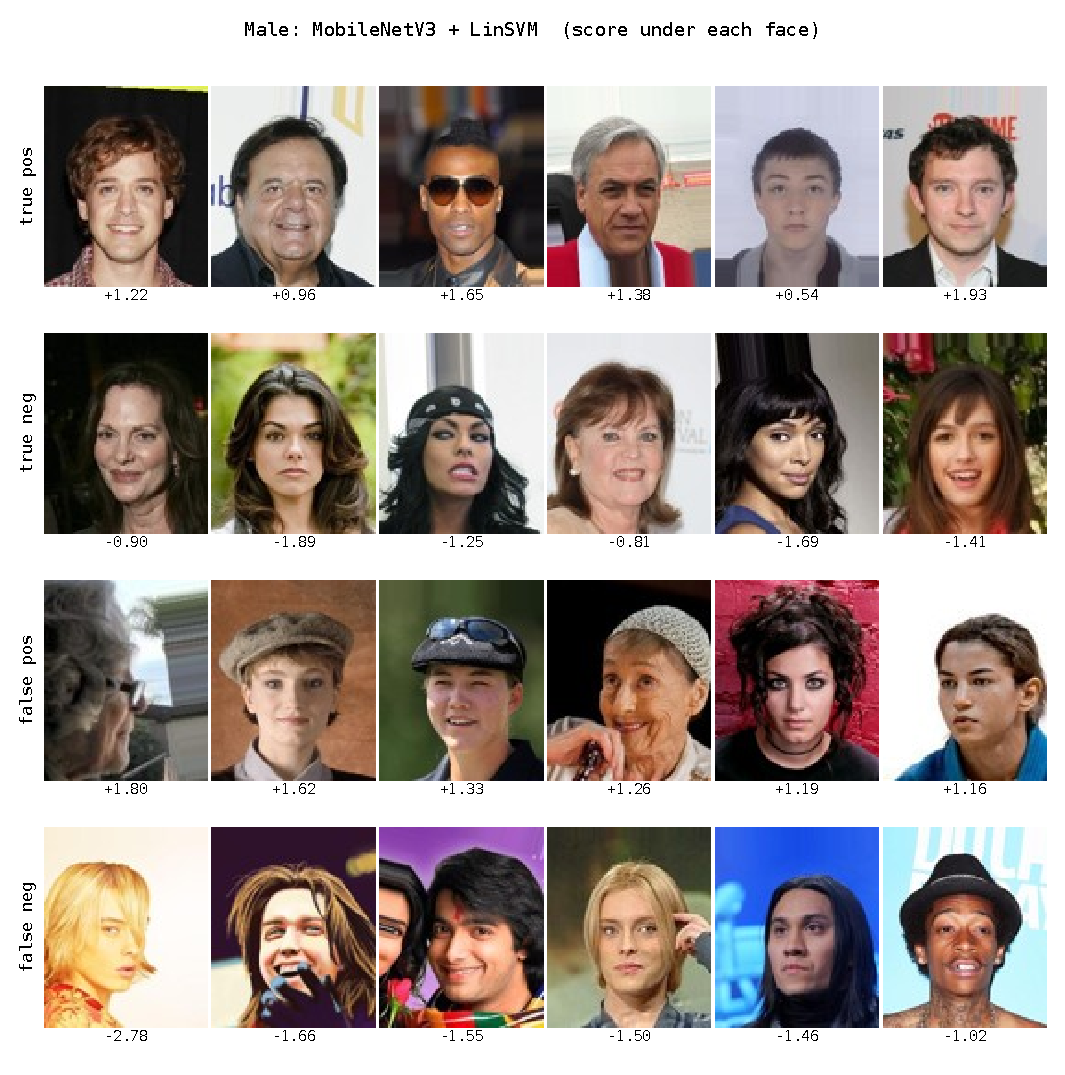
\includegraphics[width=0.84\textwidth]{figures/gallery_Male.pdf}
  \caption[Qualitative prediction gallery for Male]{Qualitative prediction gallery for \code{Male} (\code{MobileNetV3 + LinearSVC}) showing random TP/TN samples and the six most confident FP/FN errors (\code{results/\allowbreak{}figures/\allowbreak{}gallery\_\allowbreak{}Male.pdf}).}
  \label{fig:gallery_Male}
\end{figure}

\textbf{3. \code{Smiling} --- symmetric errors driven by boundary subjectivity and non-frontal poses (Figure~\ref{fig:gallery_Smiling}).}
\code{Smiling} is the hardest of the three targets (F1 = 0.7962, ROC-AUC = 0.8781), exhibiting an exactly symmetric confusion matrix (403 FP and 403 FN). Unlike \code{Eyeglasses} or \code{Male}, general ImageNet object features are less specialized for subtle facial-muscle action units:
\begin{itemize}[leftmargin=18pt, itemsep=1.5pt]
  \item \emph{False positives} (scores 0.96--0.98 despite label 0) frequently display subtle closed-mouth smiles or gently upturned lip corners, reflecting inherent annotator subjectivity at the neutral-versus-smiling boundary.
  \item \emph{False negatives} (scores 0.00--0.01 despite label 1) stem from extreme head yaw/profile views, open-mouth shouting or singing expressions with hand/microphone occlusion, or large dark sunglasses obscuring eye-crinkling cues.
\end{itemize}

\begin{figure}[H]
  \centering
  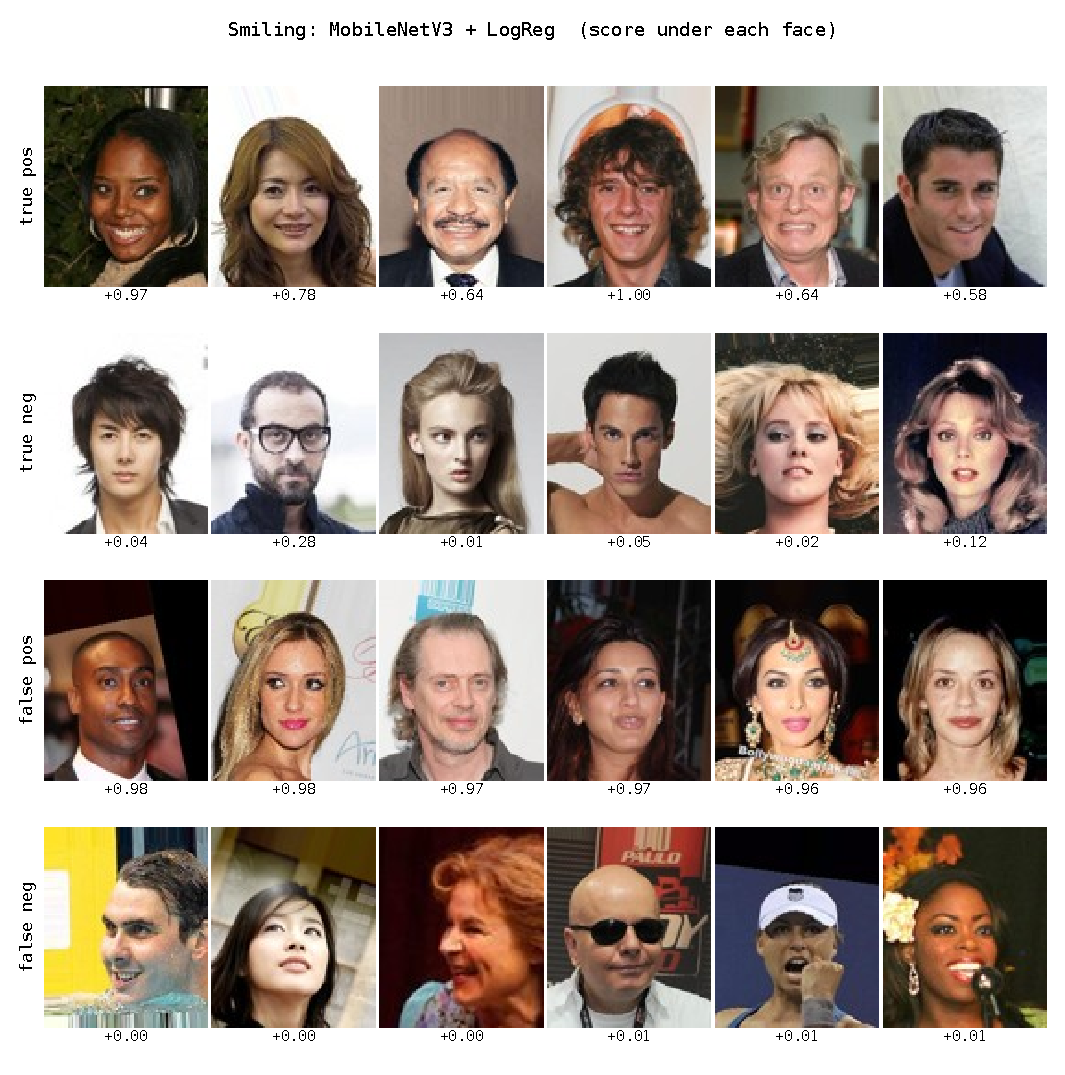
\includegraphics[width=0.84\textwidth]{figures/gallery_Smiling.pdf}
  \caption[Qualitative prediction gallery for Smiling]{Qualitative prediction gallery for \code{Smiling} (\code{MobileNetV3 + LogReg}) with predicted positive-class probabilities shown below each face (\code{results/\allowbreak{}figures/\allowbreak{}gallery\_\allowbreak{}Smiling.pdf}; the leading ``+'' sign reflects the shared signed-score formatting applied across all gallery plots).}
  \label{fig:gallery_Smiling}
\end{figure}

% --------------------------------------------------
\section{Discussion, Limitations, and Conclusion}
\label{sec:discussion}

\subsection{Key Findings and Practical Insights}
\label{subsec:findings}

Synthesizing the quantitative and qualitative results produces four actionable conclusions for image-based classical ML pipelines:
\begin{enumerate}[leftmargin=20pt, itemsep=2pt]
  \item \textbf{Backbone representation dominates downstream linear classifier choice}: MobileNetV3-Large consistently outperforms ResNet-18 across every attribute and linear model, whereas \code{LinearSVC} and \code{LogisticRegression} perform nearly identically on the same feature matrix.
  \item \textbf{Strong L2 regularization is essential for frozen CNN embeddings}: High-dimensional pooled features over 20,000 training images overfit rapidly at weak regularization ($C \ge 1.0$), especially on rare classes; searching downward into $C \in [10^{-3}, 10^{-2}]$ was decisive for generalization.
  \item \textbf{Attribute difficulty tracks visual granularity and label subjectivity}: Global structural cues (\code{Male}) and distinct accessory objects (\code{Eyeglasses}) transfer readily from ImageNet representations, whereas subtle expression semantics (\code{Smiling}) encounter an earlier linear-probe ceiling without task-specific feature adaptation.
  \item \textbf{Ranking quality can exceed thresholded classification under imbalance}: On \code{Eyeglasses}, the gap between near-ceiling ROC-AUC (0.9774) and moderate Recall (0.6948) indicates that substantial F1 gains are likely achievable purely through post-hoc threshold calibration without retraining the feature extractor.
\end{enumerate}

\subsection{Limitations and Threats to Validity}
\label{subsec:limitations}

Six methodological limitations constrain the interpretation and generality of these results:
\begin{itemize}[leftmargin=18pt, itemsep=2pt]
  \item \textbf{Subsampled dataset}: Training and evaluation used 28,000 of 202,599 images ($\approx 13.8\%$ of CelebA). Consequently, absolute test scores are not directly comparable to published benchmarks evaluated on the full 19,962-image test split.
  \item \textbf{Single random seed}: All runs used a single sampling and initialization seed (\code{seed = 42}); multi-seed mean $\pm$ standard deviation intervals were not measured, which matters most for \code{Eyeglasses} ($n_{\text{pos, test}} = 249$).
  \item \textbf{No class-imbalance mitigation}: Neither \code{class\_\allowbreak{}weight="balanced"} nor validation-based decision-threshold optimization was tested for \code{Eyeglasses}, leaving Recall visibly below Precision (0.6948 vs.\ 0.9611).
  \item \textbf{Frozen features only and linear classifiers only}: End-to-end CNN fine-tuning (deep learning extension) and non-linear classical classifiers (e.g., RBF-SVM, Random Forest) were not executed; thus we cannot quantify the exact gain from task-specific feature adaptation on \code{Smiling}.
  \item \textbf{Mirror format and identity verification}: The GPU run used PNG exports from \code{flwrlabs/\allowbreak{}celeba} rather than the original Kaggle JPEGs audited in the notebook; while official partition codes were preserved, identity disjointness (\code{celeb\_\allowbreak{}id}) was relied upon from CelebA's protocol rather than independently re-audited.
  \item \textbf{Minor geometric distortion and timing coverage}: Square resizing ($218 \times 178 \to 224 \times 224$) introduces slight horizontal stretching, and wall-clock timing was logged for CNN feature extraction (13--14\,s) but not separately for downstream classifier fitting or per-image inference latency.
\end{itemize}

\subsection{Future Work}
\label{subsec:future_work}

Four concrete extensions directly address the limitations above:
\begin{enumerate}[leftmargin=20pt, itemsep=2pt]
  \item \textbf{Imbalance-aware thresholding}: Sweep decision thresholds on the saved \code{validation\_\allowbreak{}predictions.csv} files (and compare with \code{class\_\allowbreak{}weight="balanced"}) to raise \code{Eyeglasses} Recall while controlling Precision.
  \item \textbf{Richer feature extractors and end-to-end fine-tuning}: Benchmark \code{resnet50} (already implemented in \code{extraction.py}) and Vision Transformers (ViT / Swin) alongside an end-to-end fine-tuned MobileNetV3/ResNet baseline to quantify the cost--accuracy trade-off against frozen linear probes, especially on \code{Smiling}.
  \item \textbf{Full-dataset and multi-seed evaluation}: Scale the pipeline to all 202,599 CelebA images across three random seeds to obtain tighter confidence intervals.
  \item \textbf{Non-linear classifiers and calibration}: Evaluate RBF-SVM or shallow MLPs on top of frozen features and apply Platt/isotonic probability calibration to \code{LinearSVC} margins.
\end{enumerate}

\subsection{Conclusion}
\label{subsec:conclusion}

We designed, verified, and evaluated a complete, leakage-free Machine Learning pipeline for facial-attribute classification on CelebA following Task~3 of Machine Learning (CO3117). Grounded in full-dataset EDA across 202,599 images, our 18-configuration experiment on 28,000 officially partitioned images demonstrates that frozen \textbf{MobileNetV3-Large} representations paired with strongly regularized linear classifiers deliver strong generalization across diverse attribute regimes---achieving test F1-scores of \textbf{0.8065} on \code{Eyeglasses} (\code{LinearSVC}, $C=0.001$), \textbf{0.9187} on \code{Male} (\code{LinearSVC}, $C=0.001$), and \textbf{0.7962} on \code{Smiling} (\code{LogisticRegression}, $C=0.01$)---while completing feature extraction in 13.11 seconds on a single GPU. Together, our quantitative sensitivity curves, confusion matrices, and visual error galleries pinpoint clear, evidence-backed avenues for future improvement through threshold calibration and task-specific fine-tuning.

% ==================== REFERENCES ====================
\clearpage
\addcontentsline{toc}{section}{References}
\bibliographystyle{plain}
\bibliography{references}

% ==================== APPENDICES ====================
\clearpage
\appendix

\section{Repository Structure and Reproducibility}
\label{app:repo}

All source code, configurations, unit tests, exported feature files, and experimental results are hosted on GitHub at:
\begin{center}
  \url{https://github.com/kortav0103/BTL-Machine-learning}
\end{center}

\textbf{Repository directory layout (\code{origin/\allowbreak{}main}, commit \code{6ddb47e}):}
\begin{itemize}[leftmargin=18pt, itemsep=1.5pt]
  \item \code{configs/\allowbreak{}vision/\allowbreak{}celeba.json} and \code{configs/\allowbreak{}styles/\allowbreak{}}: JSON pipeline configuration and Matplotlib manuscript styling (\code{bar.toml}, \code{heatmap.toml}).
  \item \code{modules/\allowbreak{}vision/\allowbreak{}eda/\allowbreak{}}: Modular CelebA EDA toolkit (\code{base.py}, \code{labels.py}, \code{images.py}, \code{landmarks.py}, \code{bboxes.py}, \code{eval.py}).
  \item \code{modules/\allowbreak{}vision/\allowbreak{}data/\allowbreak{}}: Deterministic manifest builder (\code{celeba.py}) and image transform (\code{preprocessing.py}).
  \item \code{modules/\allowbreak{}vision/\allowbreak{}features/\allowbreak{}}: Pretrained CNN extraction (\code{extraction.py}) and row-aligned \code{.npz} storage (\code{storage.py}).
  \item \code{modules/\allowbreak{}vision/\allowbreak{}models/\allowbreak{}} \& \code{training/\allowbreak{}}: Classifier pipelines (\code{classification.py}) and leakage-free validation grid search (\code{training/\allowbreak{}classification.py}).
  \item \code{modules/\allowbreak{}vision/\allowbreak{}evaluation/\allowbreak{}}: Test metrics (\code{classification.py}), multi-run comparison (\code{comparison.py}), error galleries (\code{gallery.py}), and portable artifact bundling (\code{bundle.py}).
  \item \code{modules/\allowbreak{}vision/\allowbreak{}run.py}, \code{plot.py}, \code{predict.py}: CLI entry points for full experiments, figure re-rendering, and single-image inference.
  \item \code{notebooks/\allowbreak{}run\_\allowbreak{}vision.ipynb}: CelebA EDA notebook (cells~1--33 executed on Kaggle CelebA) with pipeline invocation cells (cells~35--41) for experiment walkthrough and Google Colab execution.
  \item \code{results/\allowbreak{}}: Archived outputs including \code{manifest.csv}, \code{comparison.csv}, \code{eda/}, \code{features/} (\code{resnet18.npy}, \code{mobilenetv3-large-ckpt.zip}, JSON metadata), \code{figures/}, \code{gallery/}, and per-run directories containing \code{run.json}, \code{metrics.json}, \code{predictions.csv}, and \code{model.joblib}.
  \item \code{scripts/\allowbreak{}} \& \code{tests/\allowbreak{}}: Hugging Face CelebA downloader (\code{download\_\allowbreak{}celeba.py}), GPU runner (\code{vast\_\allowbreak{}run.sh}), and automated \code{pytest} suites.
  \item \code{meetings/}: Weekly meeting logs (\code{MEETINGS.md}) and collaboration records.
\end{itemize}

\vspace{4pt}
\noindent\begin{minipage}{\linewidth}
\textbf{Core reproduction commands:}
\begin{quote}
\footnotesize\ttfamily
uv sync\\
python scripts/download\_celeba.py --data-dir data\\
python -m modules.vision.run --config configs/vision/celeba.json \textbackslash\\
\hspace*{1.2em}--results-dir results\_repro --export-bundle\\
python -m modules.vision.predict \textbackslash\\
\hspace*{1.2em}results/Smiling/mobilenet\_v3\_large/logistic\_regression face.jpg\\
python -m pytest tests -q
\end{quote}
\noindent{\small\emph{Note:} Because \code{results/} is already committed in the repository, \code{--results-dir} must point to a fresh output directory whenever \code{--export-bundle} is enabled.}
\end{minipage}

\section{Complete Validation Hyperparameter Tuning Results}
\label{app:tuning}

Table~\ref{tab:full_c_grid} lists the exact validation F1-scores across all six tested regularization values ($C \in \{10^{-4},\allowbreak 10^{-3},\allowbreak 10^{-2},\allowbreak 10^{-1},\allowbreak 1.0,\allowbreak 10.0\}$) extracted directly from each configuration's \code{run.json} file on \code{origin/\allowbreak{}main}.

\begin{table}[H]
  \centering
  \caption[Full validation F1-score tuning grid across C]{Validation F1-scores across the full six-point $C$ grid for all 12 parameterized configurations ($n_{\text{val}} = 4{,}000$, \code{seed = 42}). \textbf{Bold} entries denote the selected value of $C$ per row.}
  \label{tab:full_c_grid}
  \footnotesize
  \begin{tabular}{@{}l l l r r r r r r@{}}
    \toprule
    \textbf{Target} & \textbf{Extractor} & \textbf{Classifier} & $C{=}10^{-4}$ & $C{=}10^{-3}$ & $C{=}10^{-2}$ & $C{=}0.1$ & $C{=}1.0$ & $C{=}10.0$ \\
    \midrule
    \multirow{4}{*}{\code{Eyeglasses}}
      & MobileNetV3 & LinearSVC & 0.7289 & \textbf{0.8285} & 0.8173 & 0.7491 & 0.7211 & 0.7129 \\
      & MobileNetV3 & LogReg    & 0.2848 & 0.6794 & \textbf{0.8167} & 0.8015 & 0.7572 & 0.7270 \\
      & ResNet-18   & LinearSVC & 0.6015 & 0.7169 & \textbf{0.7617} & 0.7609 & 0.7582 & 0.7592 \\
      & ResNet-18   & LogReg    & 0.2965 & 0.6522 & \textbf{0.7692} & 0.7686 & 0.7596 & 0.7575 \\
    \midrule
    \multirow{4}{*}{\code{Male}}
      & MobileNetV3 & LinearSVC & 0.9325 & \textbf{0.9329} & 0.9307 & 0.9289 & 0.9289 & 0.9289 \\
      & MobileNetV3 & LogReg    & 0.9150 & \textbf{0.9318} & 0.9317 & 0.9311 & 0.9290 & 0.9281 \\
      & ResNet-18   & LinearSVC & 0.9204 & 0.9216 & \textbf{0.9240} & 0.9231 & 0.9237 & 0.9234 \\
      & ResNet-18   & LogReg    & 0.9091 & 0.9186 & \textbf{0.9218} & 0.9210 & 0.9213 & 0.9216 \\
    \midrule
    \multirow{4}{*}{\code{Smiling}}
      & MobileNetV3 & LinearSVC & 0.7886 & \textbf{0.7951} & 0.7938 & 0.7923 & 0.7921 & 0.7921 \\
      & MobileNetV3 & LogReg    & 0.7586 & 0.7866 & \textbf{0.7959} & 0.7953 & 0.7951 & 0.7948 \\
      & ResNet-18   & LinearSVC & 0.7711 & 0.7758 & \textbf{0.7798} & 0.7774 & 0.7781 & 0.7784 \\
      & ResNet-18   & LogReg    & 0.7437 & 0.7681 & 0.7783 & \textbf{0.7794} & 0.7789 & 0.7785 \\
    \bottomrule
  \end{tabular}
\end{table}

\end{document}
